\documentclass{beamer}

\title{Mid-PhD Defense}
\author{Paul Dubois}
\institute{
	TheraPanacea\\
	MICS, CentraleSupélec\\
	Institut du Cancer de Montpellier
}
\date{21st June 2023}

\usepackage{tikz}
\usepackage{multicol}
\usepackage{nicefrac}
\usepackage[justification=centering]{subfig}

\begin{document}
	
	\frame{\titlepage}
	
	\begin{frame}
		\frametitle{Outline}
		\begin{multicols}{2}
			\tableofcontents
		\end{multicols}
	\end{frame}

	\section{Introduction}
	\subsection{Cancer treatments}
	\begin{frame}
		\makebox[\linewidth]{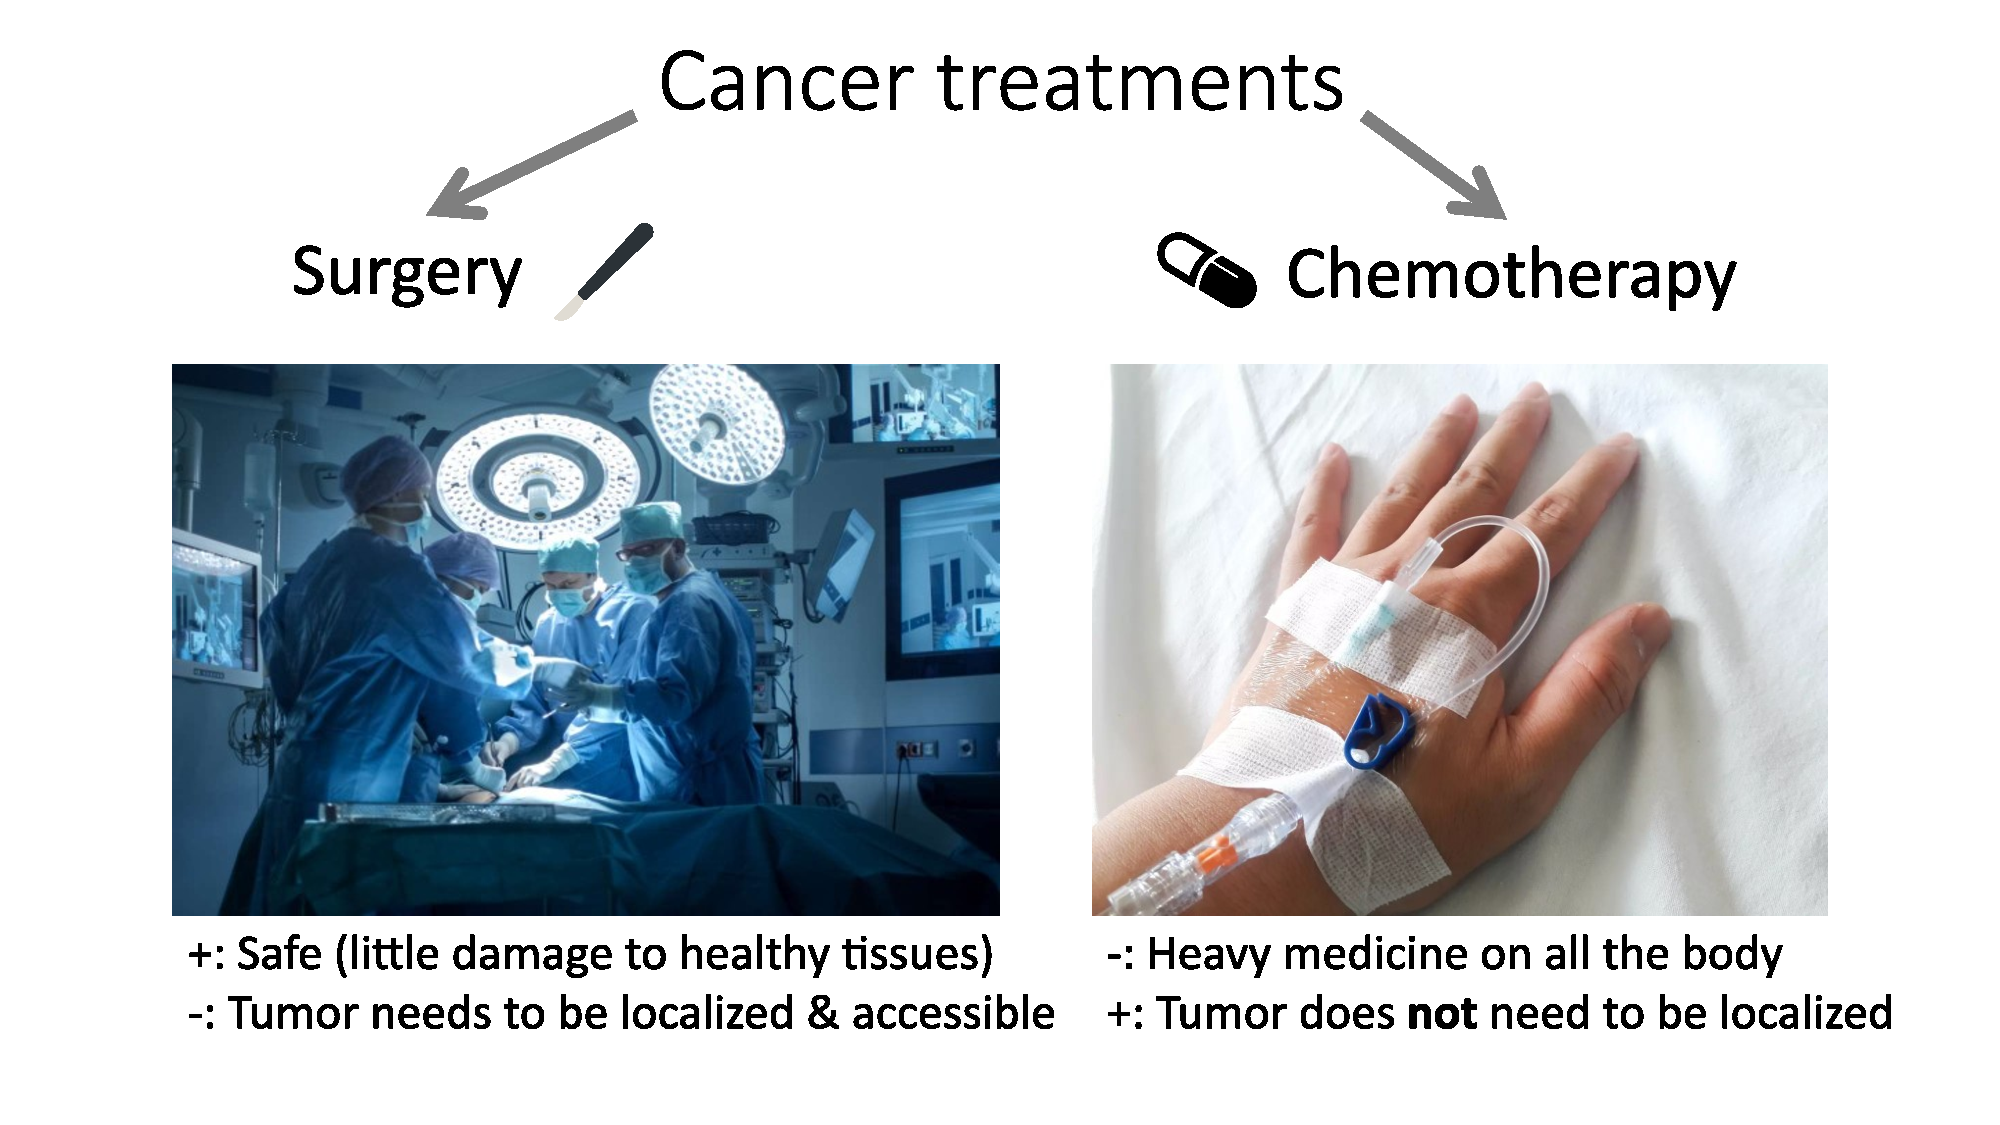
\includegraphics[width=\paperwidth]{imported_slides/cancer_treatments.pdf}}
	\end{frame}
	
	\subsection{Radiotherapy}
	\begin{frame}
		\makebox[\linewidth]{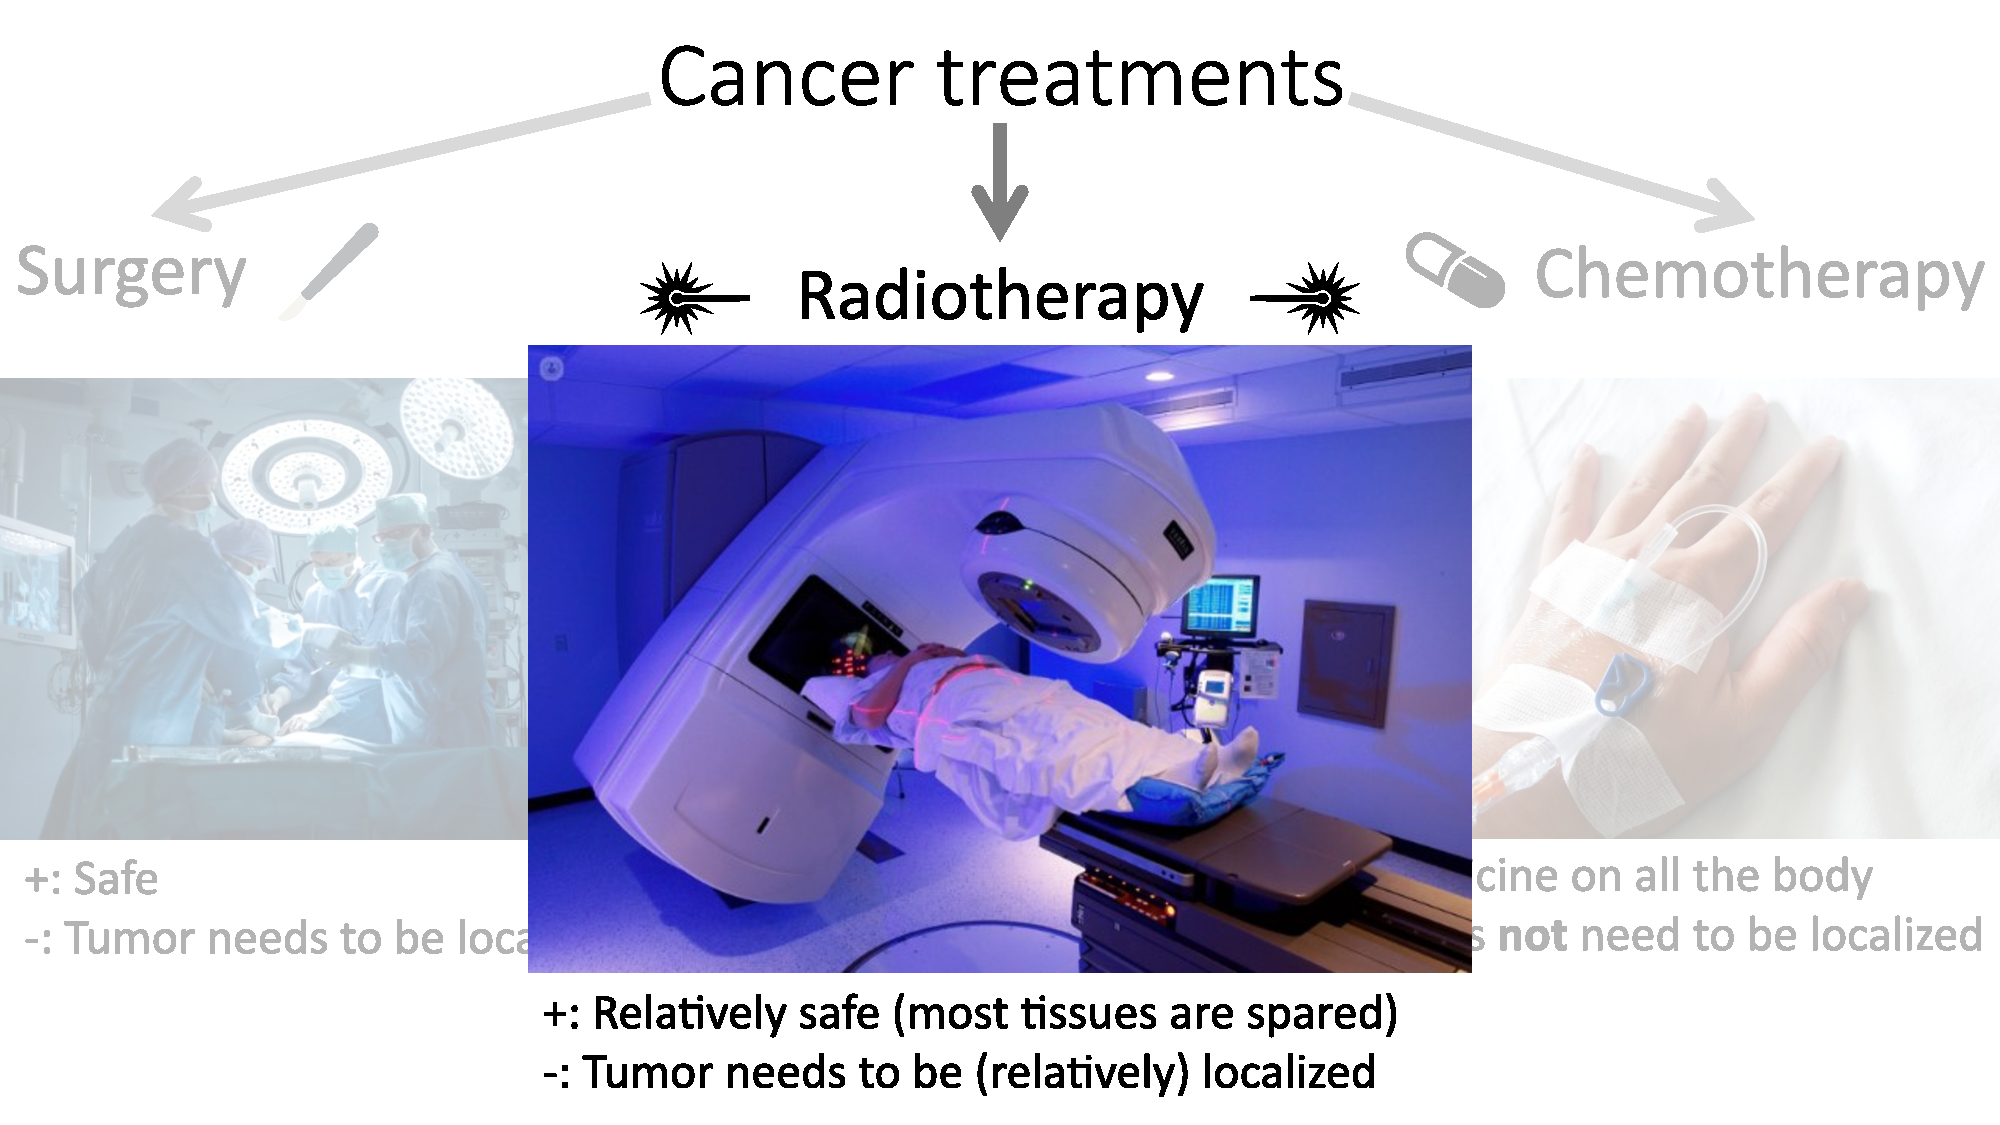
\includegraphics[width=\paperwidth]{imported_slides/cancer_treatments_bis.pdf}}
	\end{frame}
	
	\subsection{Multi-Leaf Collimator}
	\begin{frame}
		\frametitle{Multi-Leaf Collimator}
		\makebox[\linewidth]{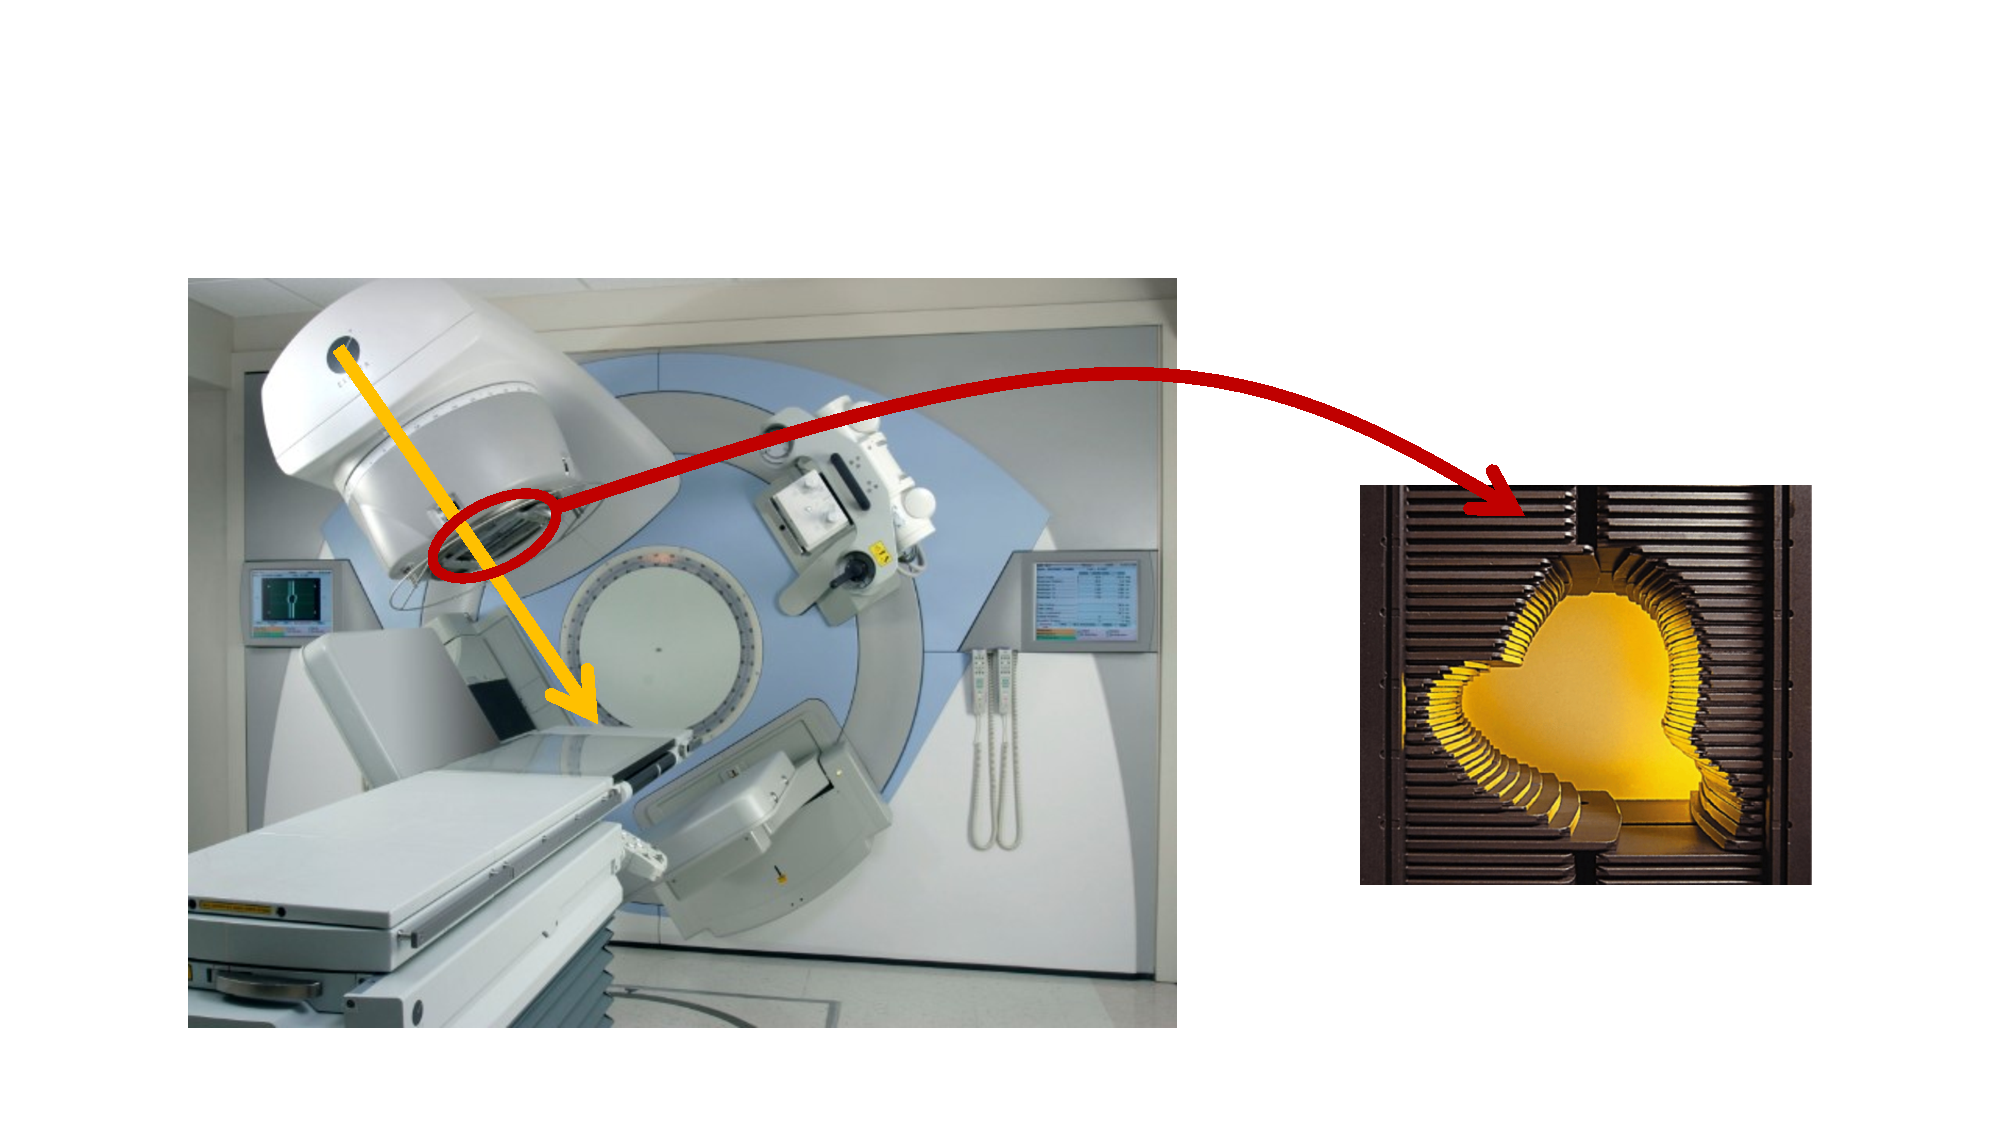
\includegraphics[width=\paperwidth]{imported_slides/multi_leaf_collimator.pdf}}
	\end{frame}
	
	\subsection{V-MAT Scheme}
	\begin{frame}
		\frametitle{V-MAT Irradiation Technique}
		\begin{figure}
			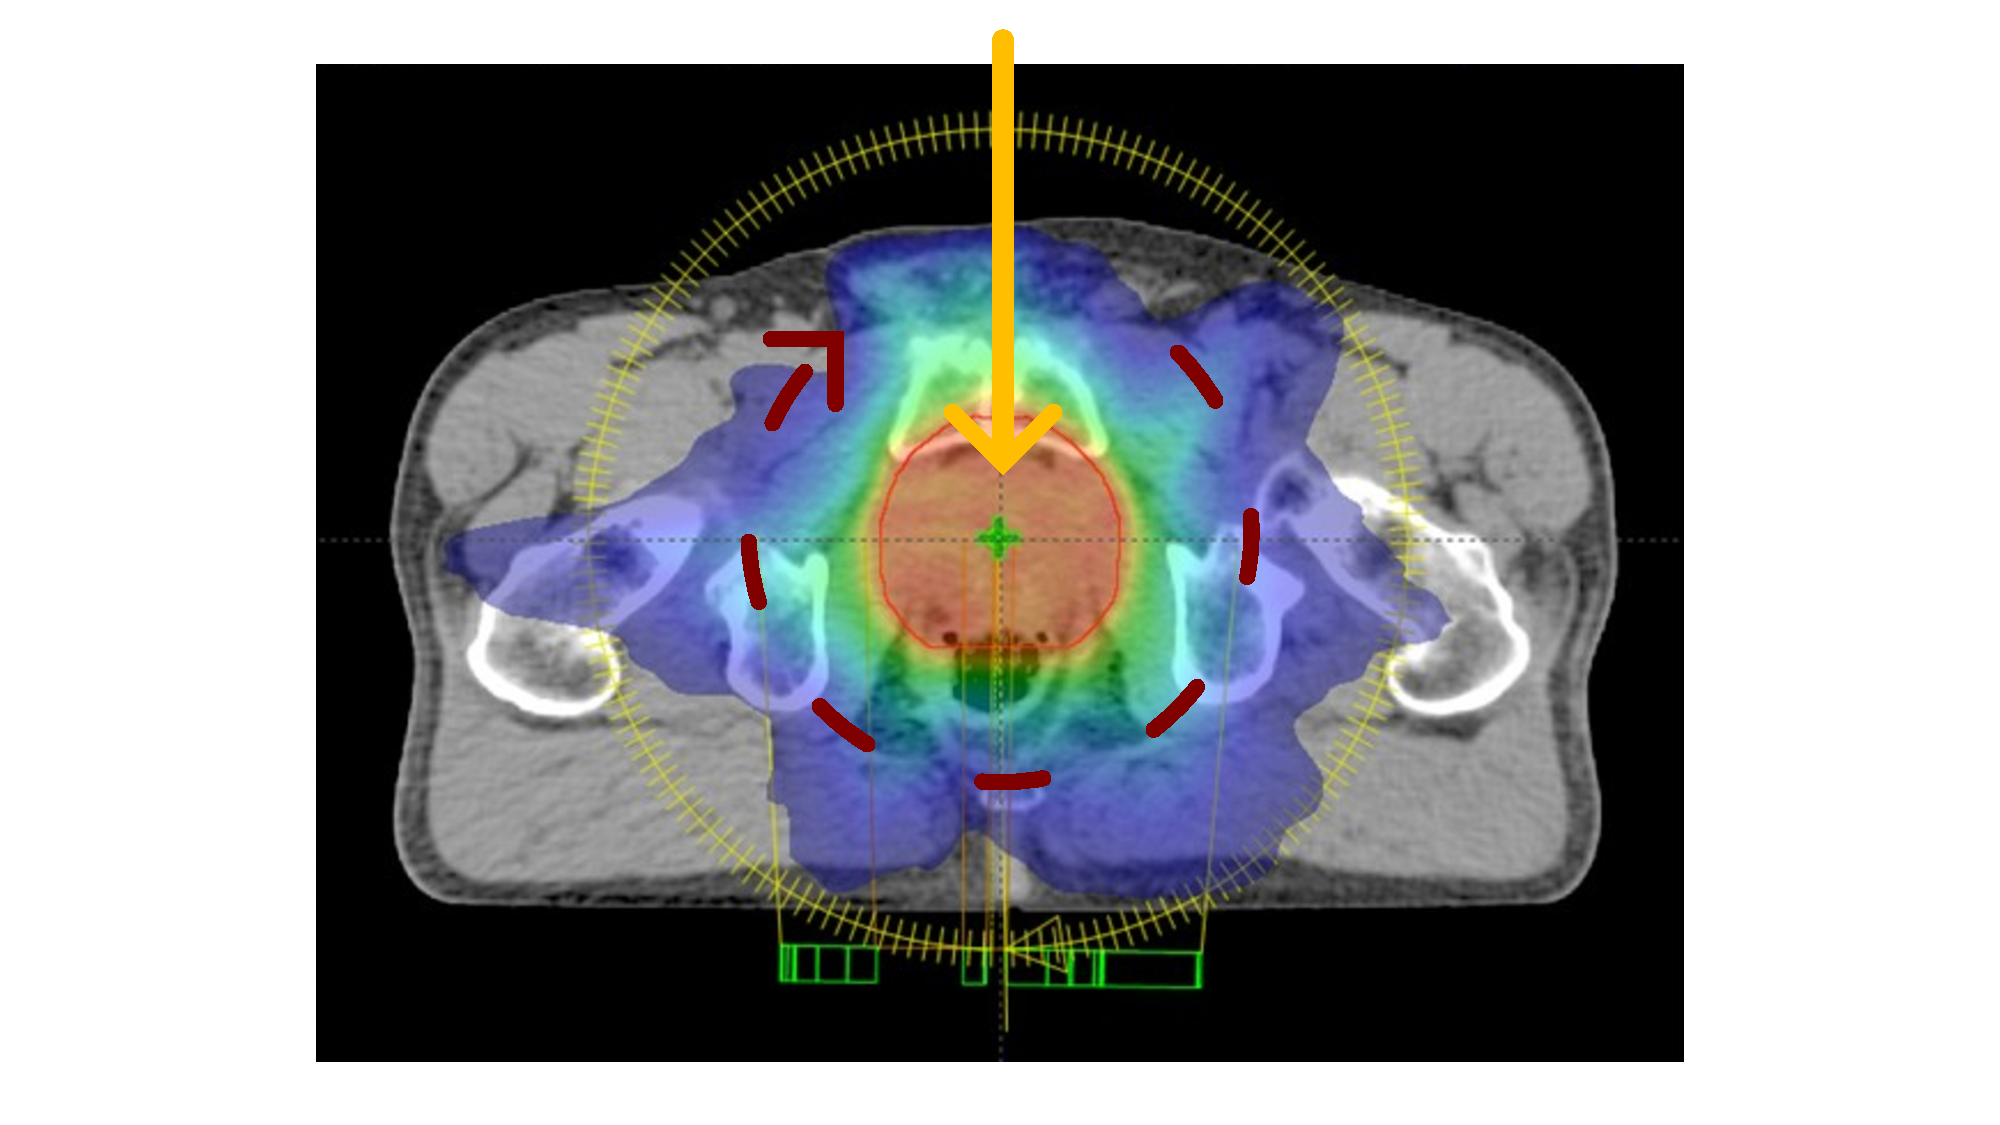
\includegraphics[height=6cm]{vector_images/example_dose_vmat_arrows.pdf}
			\caption{Typical V-Mat dose slice.}
		\end{figure}
	\end{frame}
	
	\subsection{IMRT Scheme}
	\begin{frame}
		\frametitle{IMRT Irradiation Technique}
		\begin{figure}
			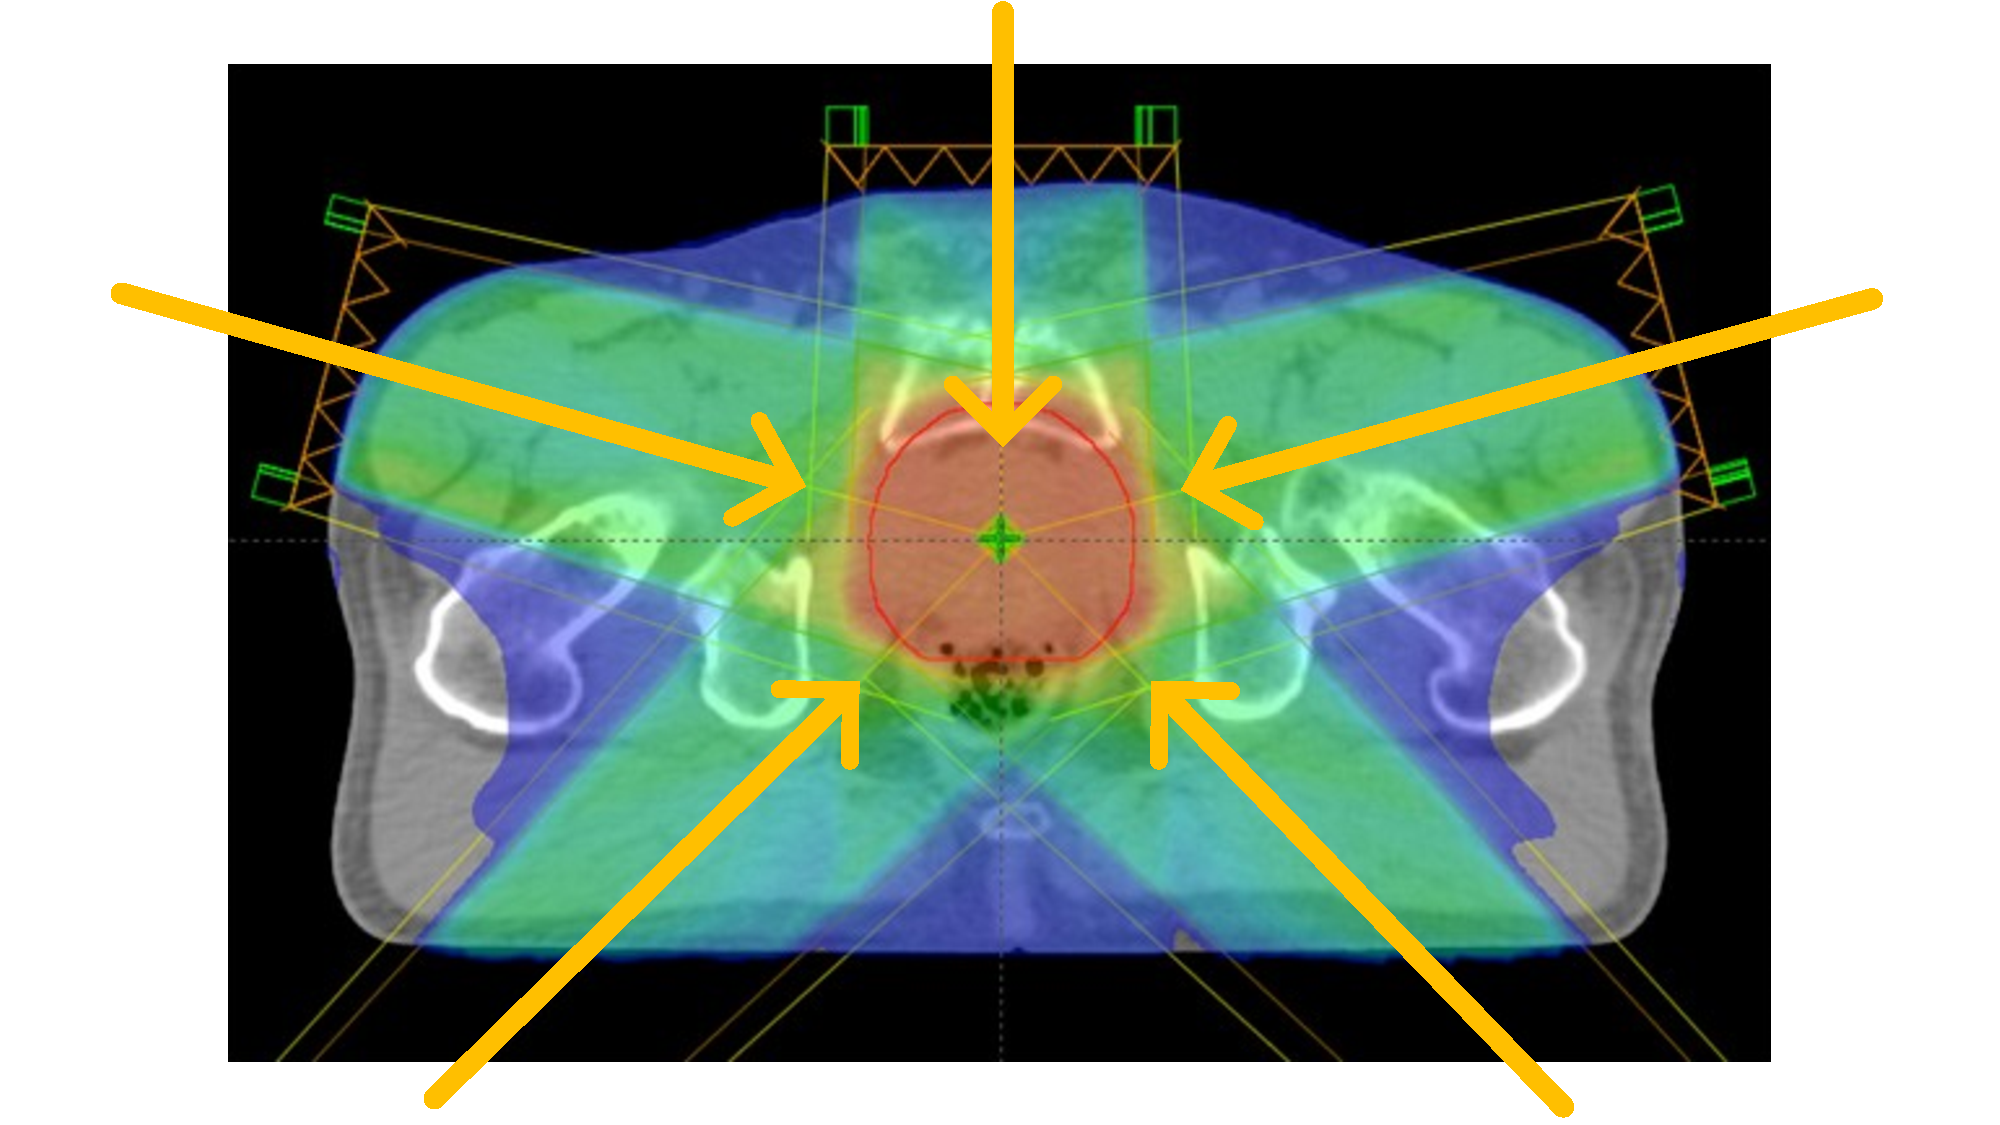
\includegraphics[height=6cm]{vector_images/example_dose_imrt5_arrows.pdf}
			\caption{Typical 5 beams IMRT dose slice.}
		\end{figure}
	\end{frame}
	
	\subsubsection{Step-and-Shoot}
	\begin{frame}
		\frametitle{Step-and-Shoot (1/3)}
		\begin{figure}
			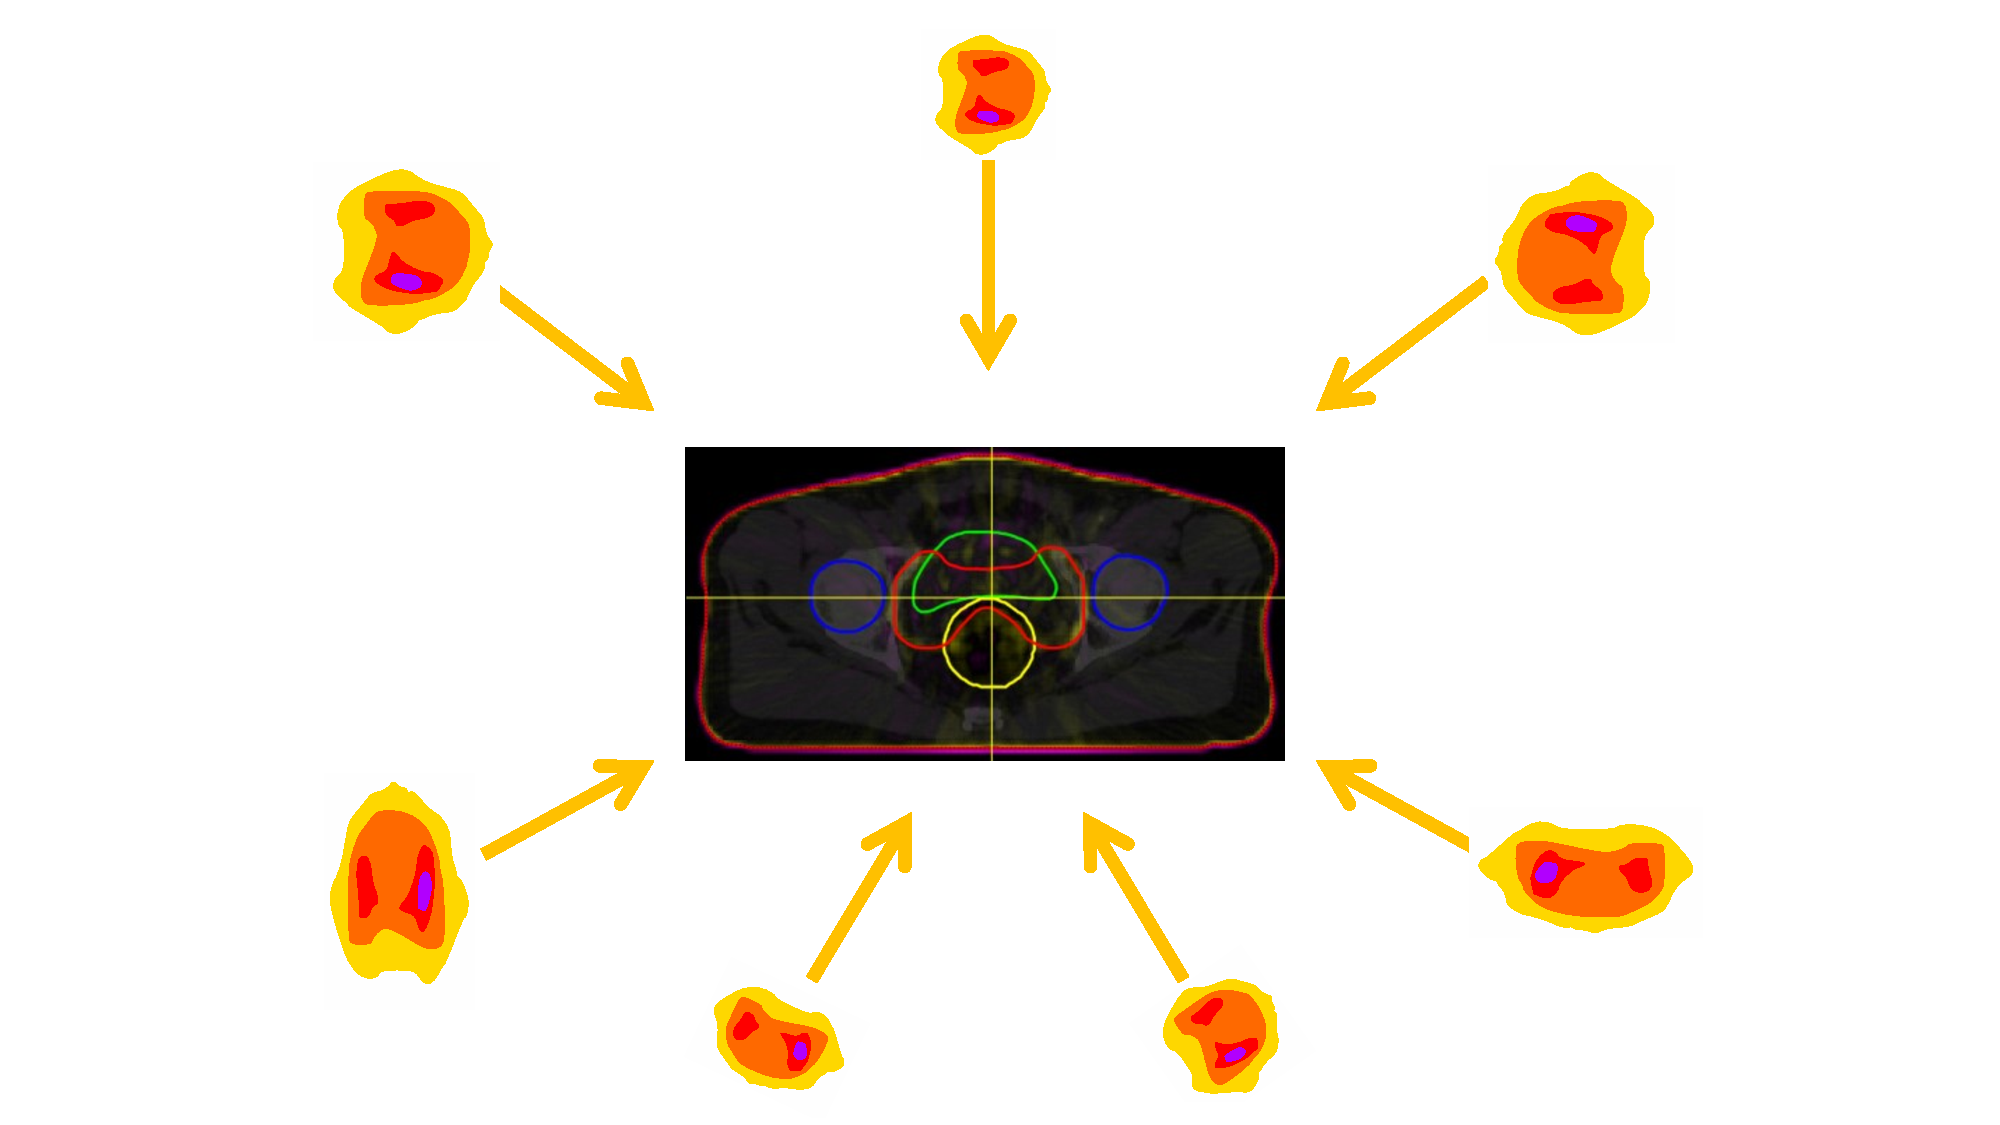
\includegraphics[height=6cm]{vector_images/optimal_fluences.pdf}
			\caption{Optimal Continuous Fluence.}
		\end{figure}
	\end{frame}
	\begin{frame}
	\frametitle{Step-and-Shoot (2/3)}
	\begin{figure}
		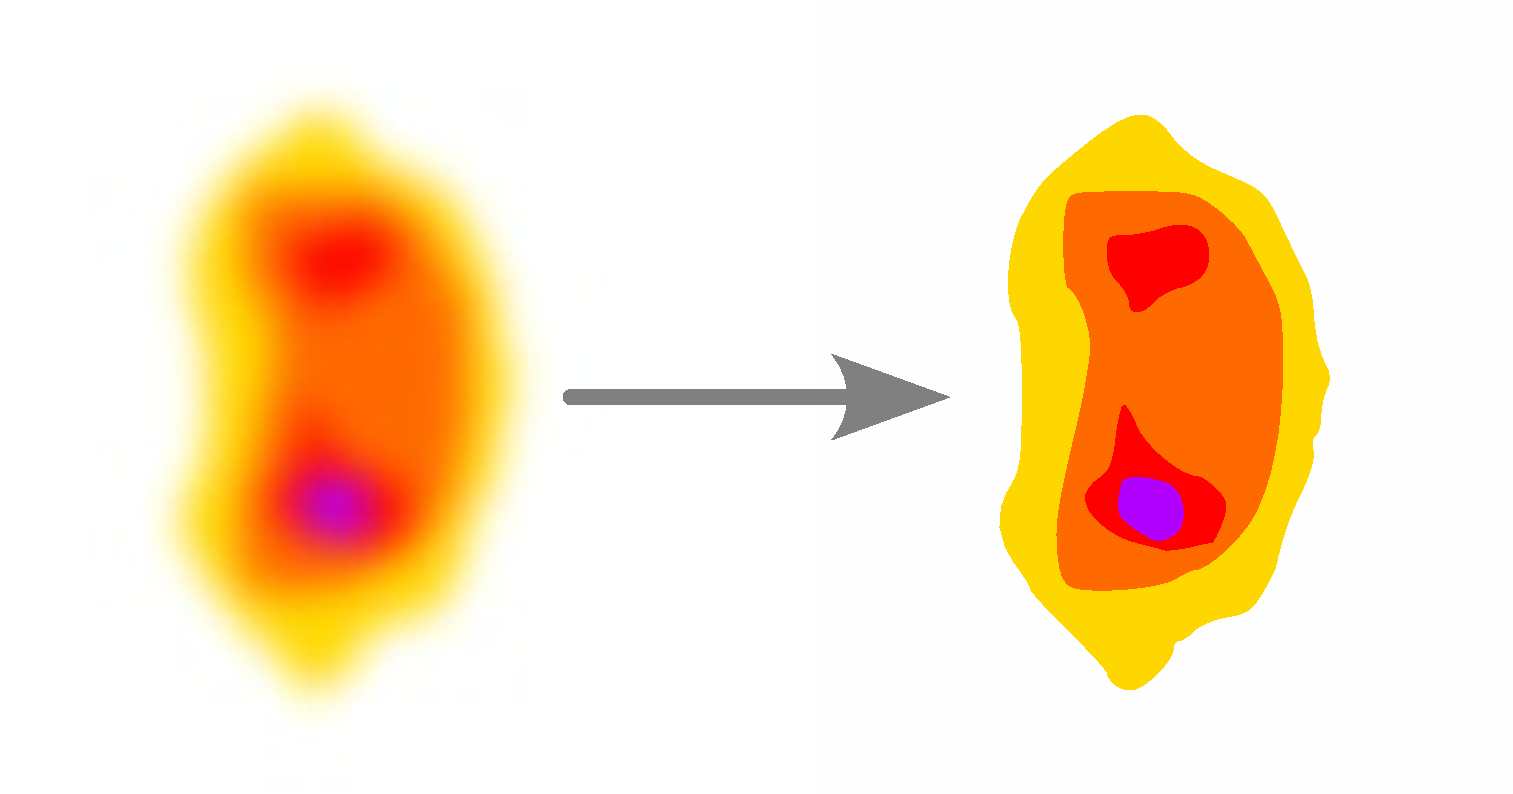
\includegraphics[width=\linewidth]{vector_images/fluence_discretization.pdf}
		\caption{Discretizing the Fluence.}
	\end{figure}
	\end{frame}
	\begin{frame}
		\frametitle{Step-and-Shoot (3/3)}
		\begin{figure}
			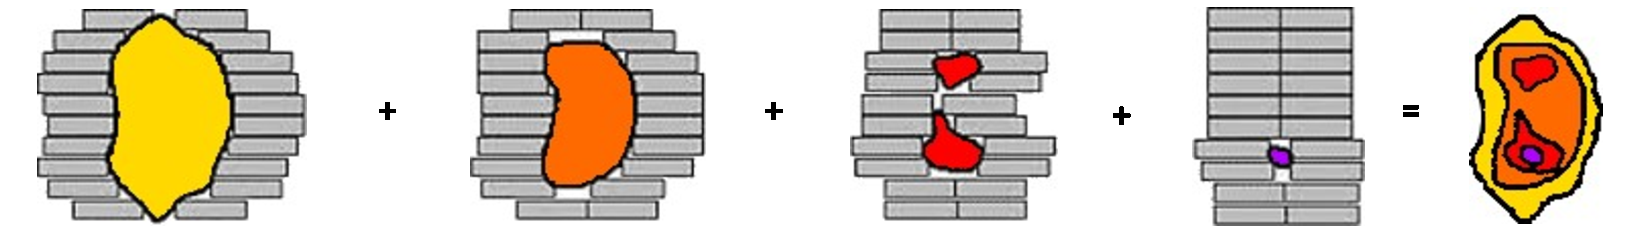
\includegraphics[width=\linewidth]{vector_images/step_and_shoot.pdf}
			\caption{Delivering Discrete Fluence.}
		\end{figure}
	\end{frame}
	
	\subsubsection{Sliding-windows}
	\begin{frame}
		\frametitle{Sliding-Windows (1/3)}
		\begin{figure}
			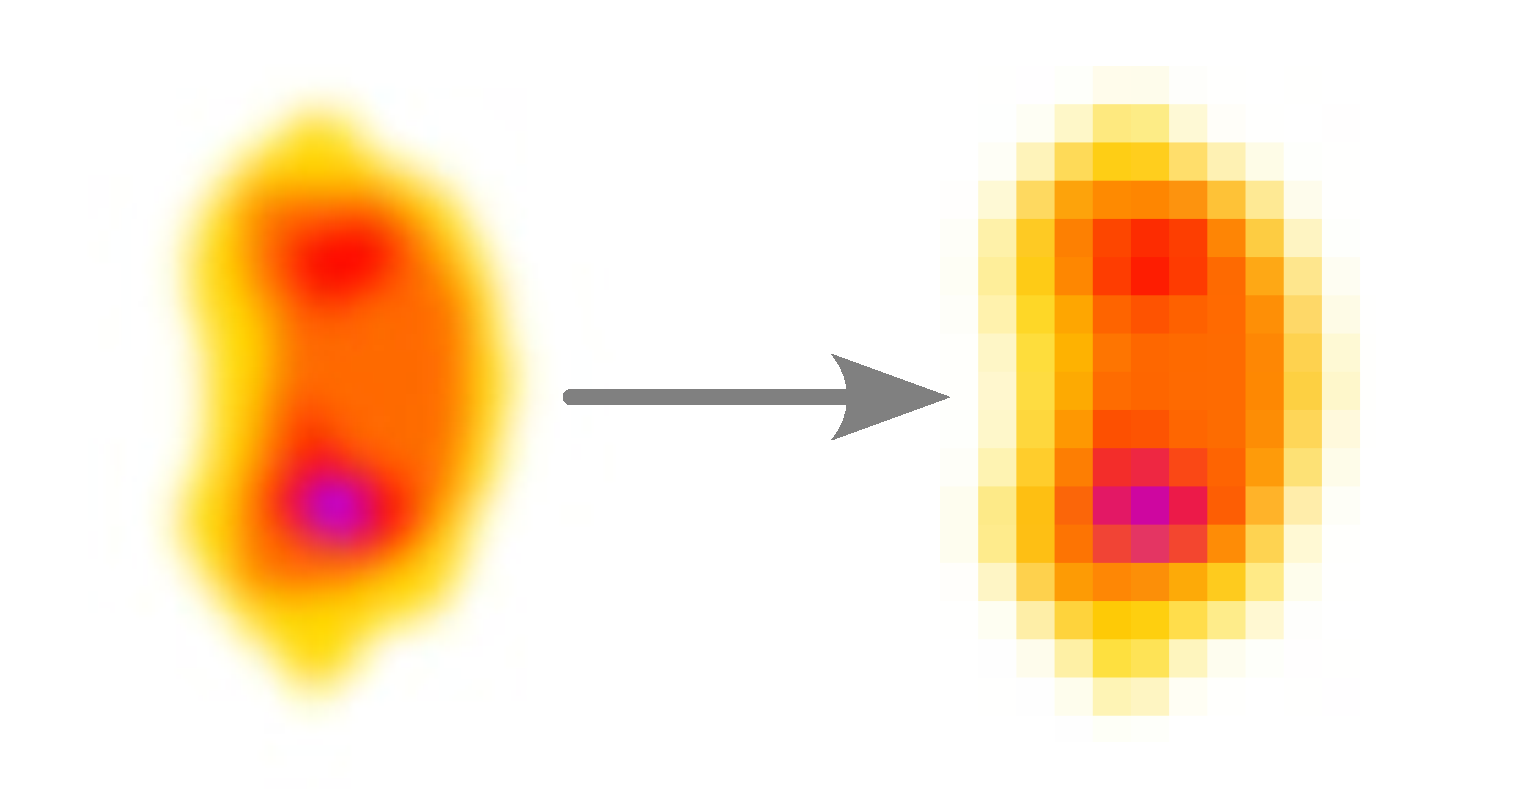
\includegraphics[width=\linewidth]{vector_images/fluence_bixelization.pdf}
			\caption{Continuous Fluence to Bixel Fluence.}
		\end{figure}
	\end{frame}
	\begin{frame}
		\frametitle{Sliding-Windows (2/3)}
		\begin{figure}
			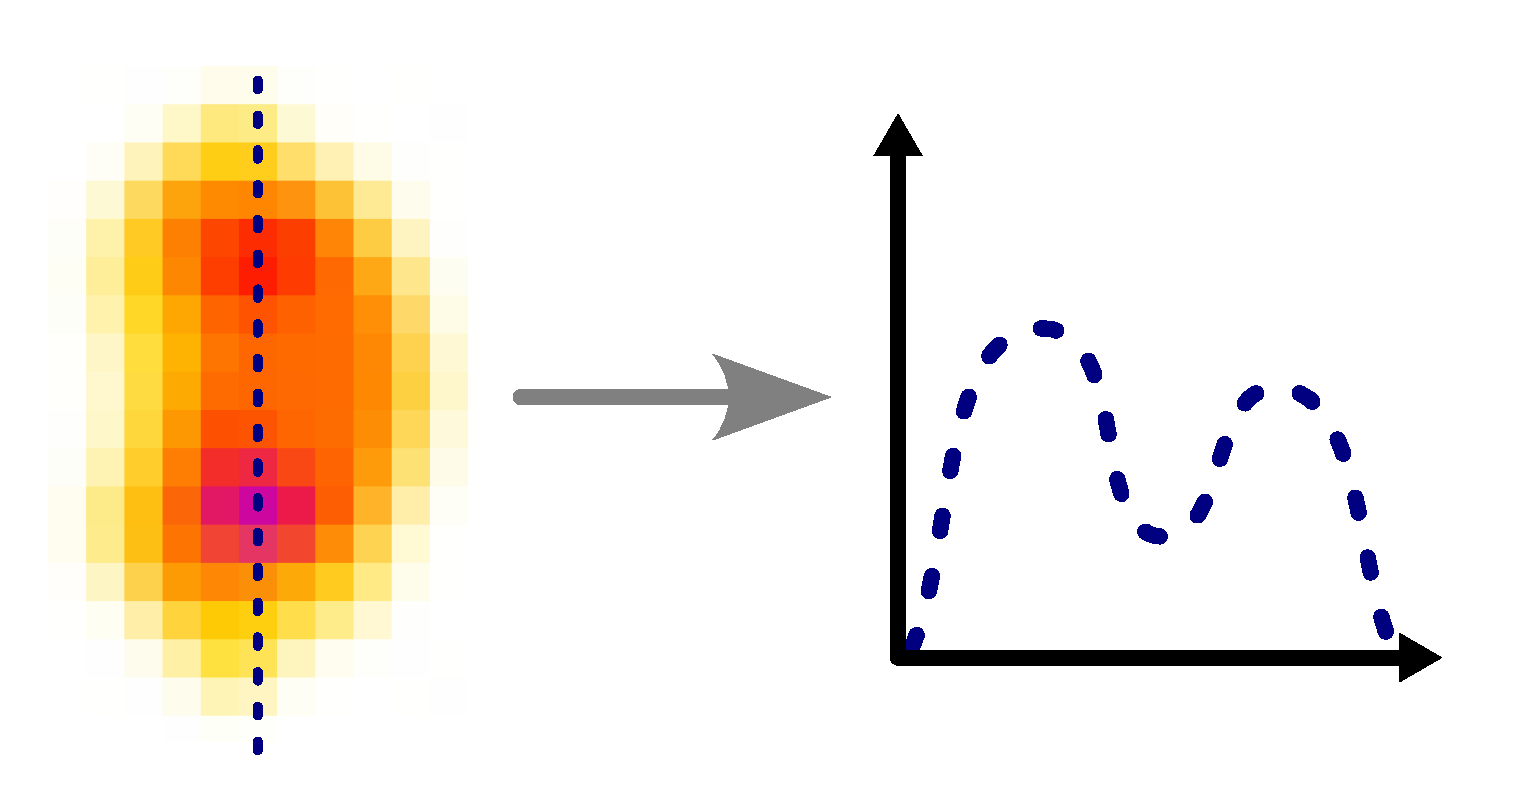
\includegraphics[width=\linewidth]{vector_images/sliding_window_curve.pdf}
			\caption{Bixel Fluence to Row/Column Curves.}
		\end{figure}
	\end{frame}
	\begin{frame}
		\frametitle{Sliding-Windows (3/3)}
		Convert rows/columns fluence curves to leafs motions.
		\begin{figure}
			
\includegraphics[height=4cm]{matrix_images/demo_QR_code.png}
		\end{figure}
		{\small (\url{https://mics-lab.github.io/PresentationJuin2023MICS/demo})}
	\end{frame}
	
	\subsection{Radiotherapy Workflow}
	\begin{frame}
		\frametitle{Radiotherapy Workflow}
		\begin{figure}
			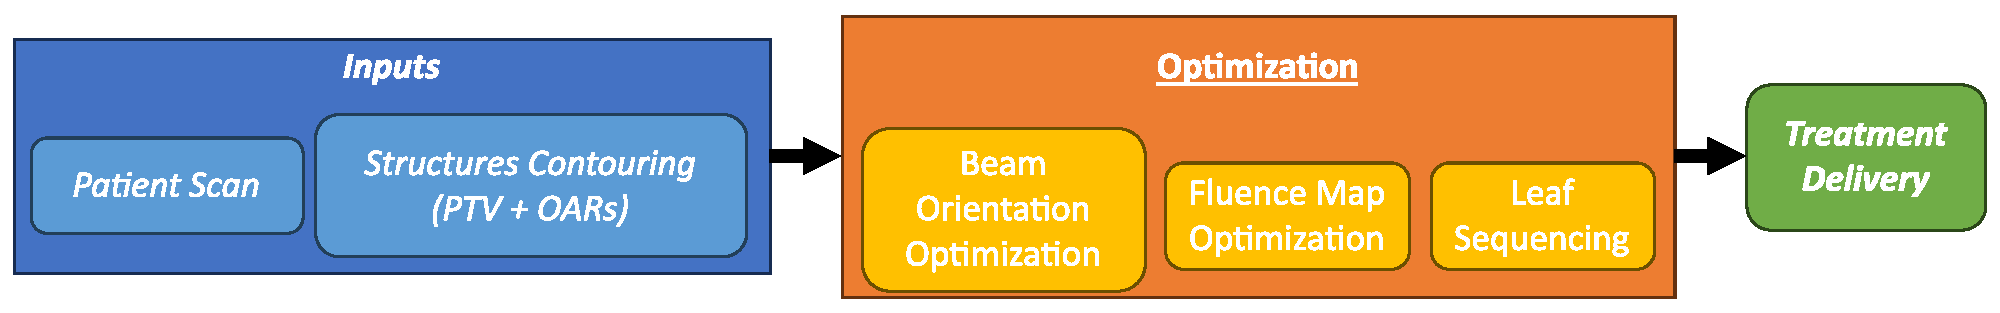
\includegraphics[width=\linewidth]{vector_images/rt_workflow.pdf}
		\end{figure}
	\end{frame}
	\begin{frame}
		\frametitle{Radiotherapy Workflow}
		\begin{figure}
			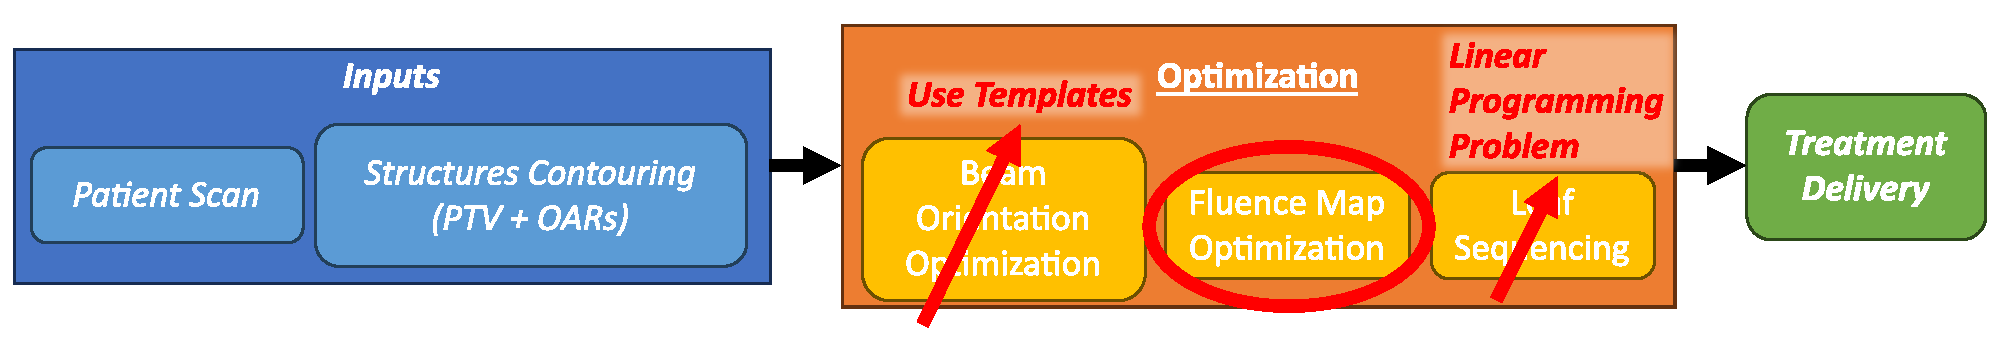
\includegraphics[width=\linewidth]{vector_images/rt_workflow_bis.pdf}
		\end{figure}
	\end{frame}
	
	\section{Problem Statement}
	\subsection{Optimization workflow}
		\begin{frame}
		\frametitle{Automatic Dose Optimization for Radiotherapy}
		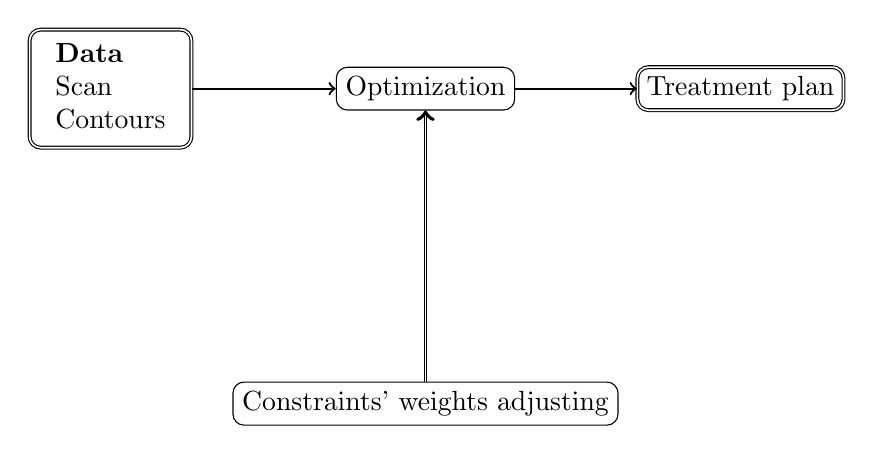
\begin{tikzpicture}[node distance=4cm]
			\node (inputs) [draw,double,rounded corners] {\begin{tabular}{l} \textbf{Data} \\ Scan \\ Contours \end{tabular}};
			\node (process) [right of=inputs,draw,rounded corners] {Optimization};
			\node (outputs) [right of=process,draw,double,rounded corners] {Treatment plan};
			\draw [thick,->] (inputs) -- (process);
			\draw [thick,->] (process) -- (outputs);
			\node (human) [below of=process,draw,rounded corners] {Constraints' weights adjusting};
			\draw [double,<-] (process) -- (human);
		\end{tikzpicture}
	\end{frame}
	
	\subsection{Fluence discretization}
	% fluence to bixels
	
	\subsection{FMO problem}
	\subsubsection{Formulation}
		\begin{frame}
		\frametitle{Problem Formulation}
		\framesubtitle{IMRT}
		Bixel values:
		$$x_{i,j}^\theta \geq 0 \text{, for } \theta \in \Theta \text{ and } 1\leq i,j \leq 20\footnote{20x20 is a typical bixel discretization}$$
		usually concatenated to a single bixels-value vector $x$.
		\vspace{0.5cm}
		
		Dose calculation:
		$$\textbf{y} = L\textbf{x} \text{ with } L \text{ (pre-calculated) dose-influence (DI) matrix}$$
	\end{frame}
	\begin{frame}
		\frametitle{Problem Formulation}
		\framesubtitle{IMRT (bis)}
		Objective for \textit{maximum} constraint $c$ on structure $s$, dose $d$:
		$$f_c(\textbf{y}) = \frac{1}{|\mathcal{V}|} \sum_{v \in \mathcal{V}} (\textbf{y}_v-d)_+^2$$
		(reverse sign for minimal constraint).
		\vspace{0.5cm}
		
		Final objective:
		$$f(\textbf{y}) = \sum_{c \in \mathcal{C}} w_c f_c(\textbf{y})$$
		with $w_c$ the weight of constraint $c$.
	\end{frame}
	
	\subsubsection{Optimization}
	% DI matrix generation
	
	\section{Early results}
	\subsection{Optimizers Review}
	\begin{frame}
		\frametitle{Problem Optimization}
		\framesubtitle{Optimizer review}
		\begin{figure}
			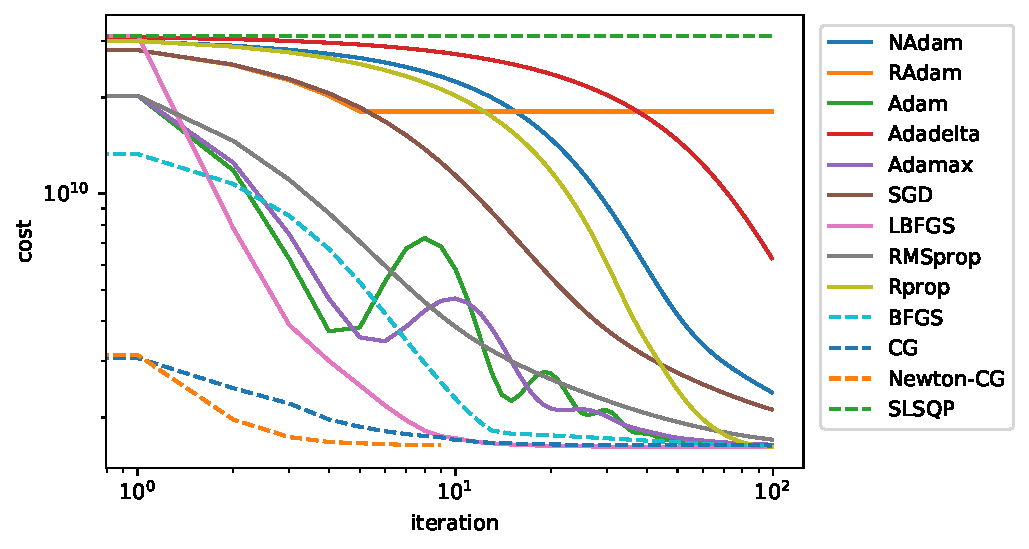
\includegraphics[width=10.75cm]{figures/ICMProstate-iter.pdf}
			\caption{Typical prostate case.}
		\end{figure}
		\url{https://arxiv.org/abs/2305.18014}
	\end{frame}
	\begin{frame}
		\frametitle{Problem Optimization}
		\framesubtitle{Optimizer review (bis)}
		\begin{figure}
			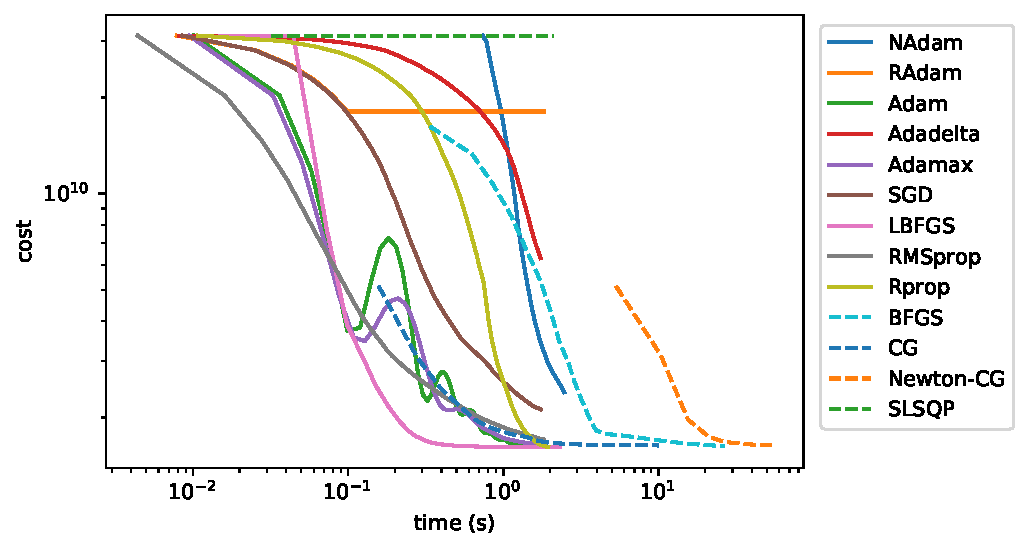
\includegraphics[width=10.75cm]{figures/ICMProstate-time.pdf}
			\caption{Typical prostate case.}
		\end{figure}
		\url{https://arxiv.org/abs/2305.18014}
	\end{frame}
	
	\subsection{Meta-Optimization}
	\begin{frame}
		\frametitle{Meta-Optimization}
		\textbf{Usual optimization}
		$$\min_{\textbf{x}} f(\textbf{x}, w) \text{ s.t. } \textbf{x} > 0$$
		... and fine-tune $w$ until the dose is clinically acceptable.
		\vspace{0.5cm}
		
		\textbf{Meta optimization}
		$$\min_w \left\lbrace \min_{\textbf{x}} f(\textbf{x}, w) \text{ s.t. } \textbf{x} > 0 \right\rbrace $$
		... still need to fine-tune the parameters (learning rate, momentum, etc...) of the meta-optimizer.
	\end{frame}
	
	\subsection{Dose Distances}
	\begin{frame}
		\frametitle{Dose Distances}
		\begin{figure}
			\vspace{-0.5cm}
			\includegraphics[width=5cm]{figures/example\_bixels.pdf}
			\includegraphics[width=5cm]{figures/example\_3d\_doses.pdf}
			\vspace{-0.3cm}
			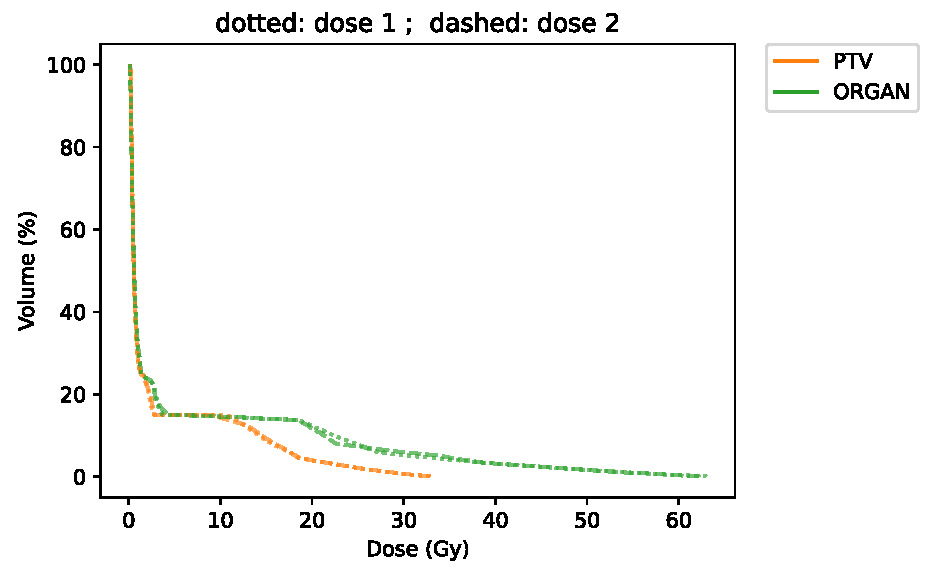
\includegraphics[width=6cm]{figures/example_dvh.pdf}
			\caption{Example of two doses that have the same clinical effect (measured from the DVHs), but very different voxel-wise dose values.}
		\end{figure}
	\end{frame}
	\subsection{Dose Clustering}
	\begin{frame}
		\frametitle{Dose Clustering}
		\begin{figure}
			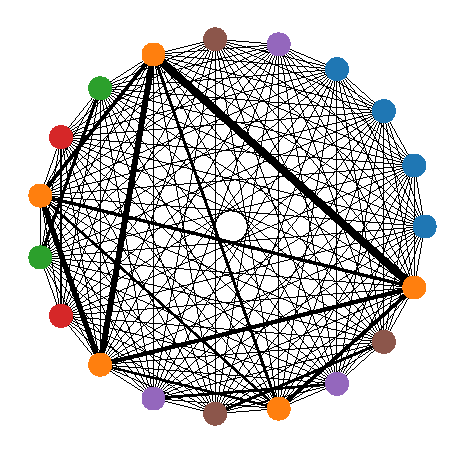
\includegraphics[width=0.35\linewidth]{figures/graph.pdf}
			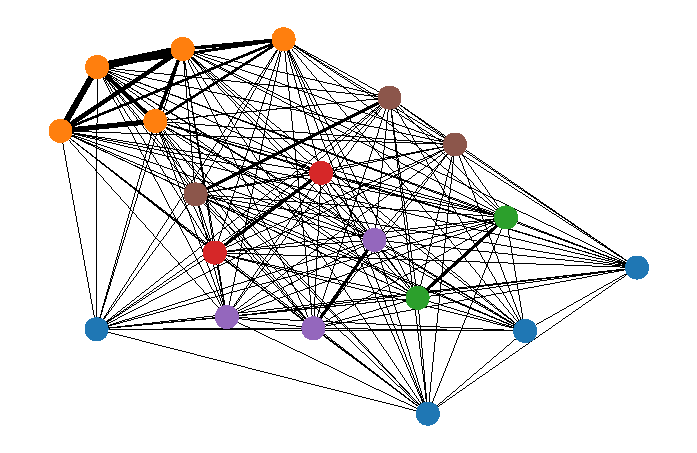
\includegraphics[width=0.54\linewidth]{figures/graph_bis.pdf}
			\subfloat[(Circular Layout)]{\hspace{.5\linewidth}}
			\subfloat[(Spring Layout)]{\hspace{.5\linewidth}}
			\caption{Doses Network}
		\end{figure}
		edges width $\propto$ edge weight $\propto$ $\nicefrac{\text{1}}{\text{distance}}$\\
		node's color reflects community attribution
	\end{frame}
	\begin{frame}
		\frametitle{Dose Clustering}
		\begin{figure}
			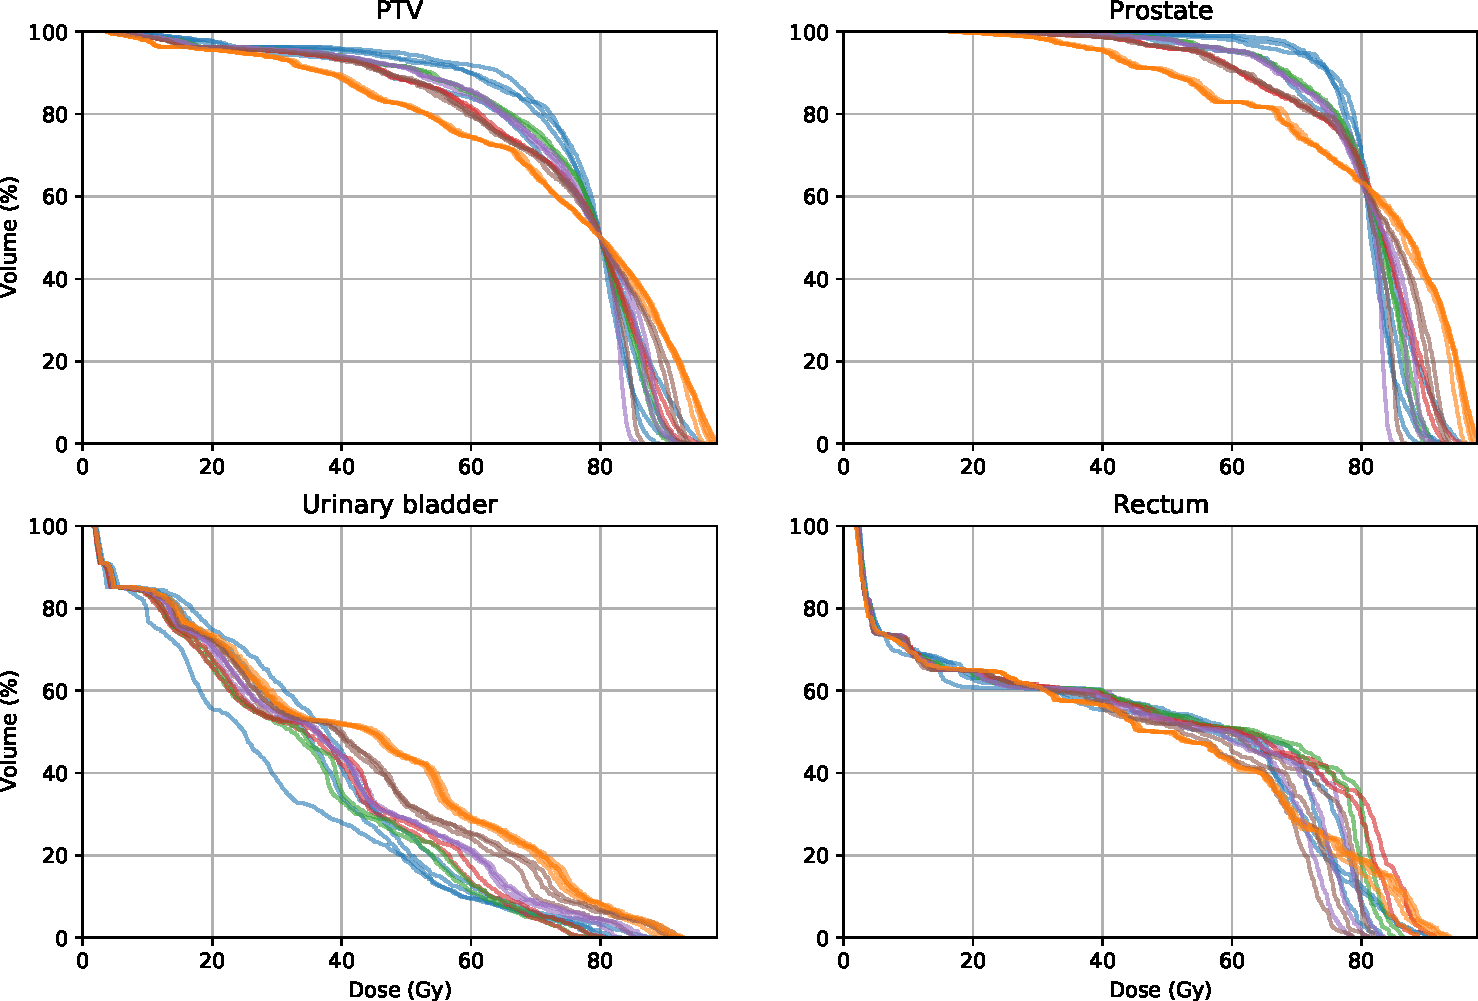
\includegraphics[width=\linewidth]{figures/dvh.pdf}
			\caption{Dose-Volume Histogram}
		\end{figure}
	\end{frame}
	\begin{frame}
		\frametitle{Dose Clustering}
		\begin{figure}
			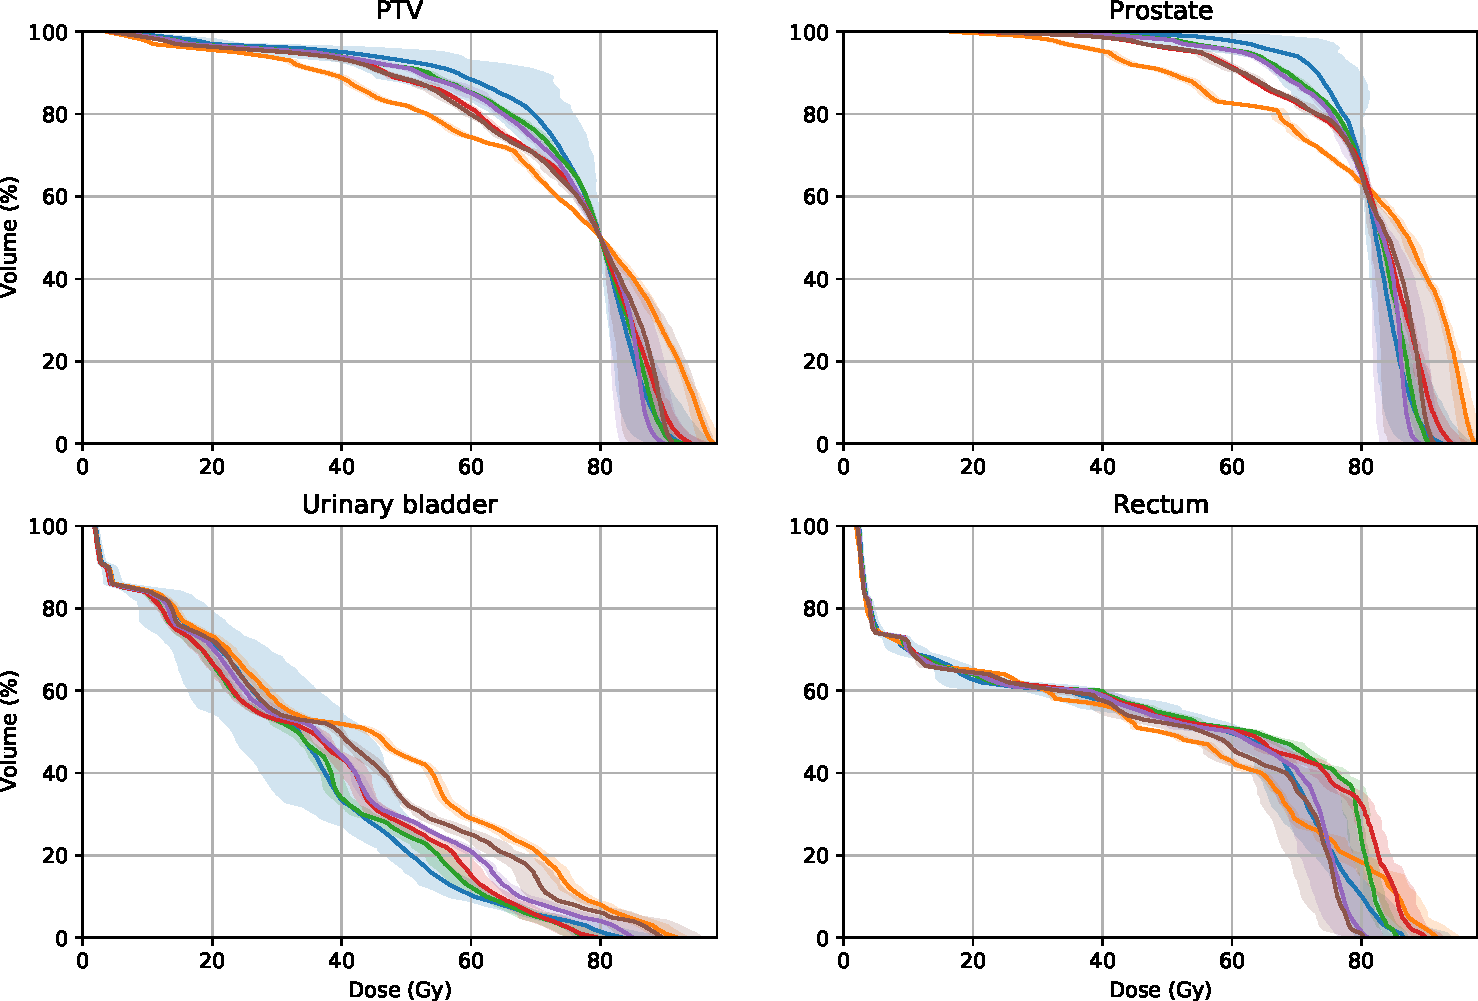
\includegraphics[width=\linewidth]{figures/dvh_std.pdf}
			\caption{Dose-Volume Histogram Standard Deviation per Community}
		\end{figure}
	\end{frame}
	
	% summary
	\begin{frame}
		\makebox[\linewidth]{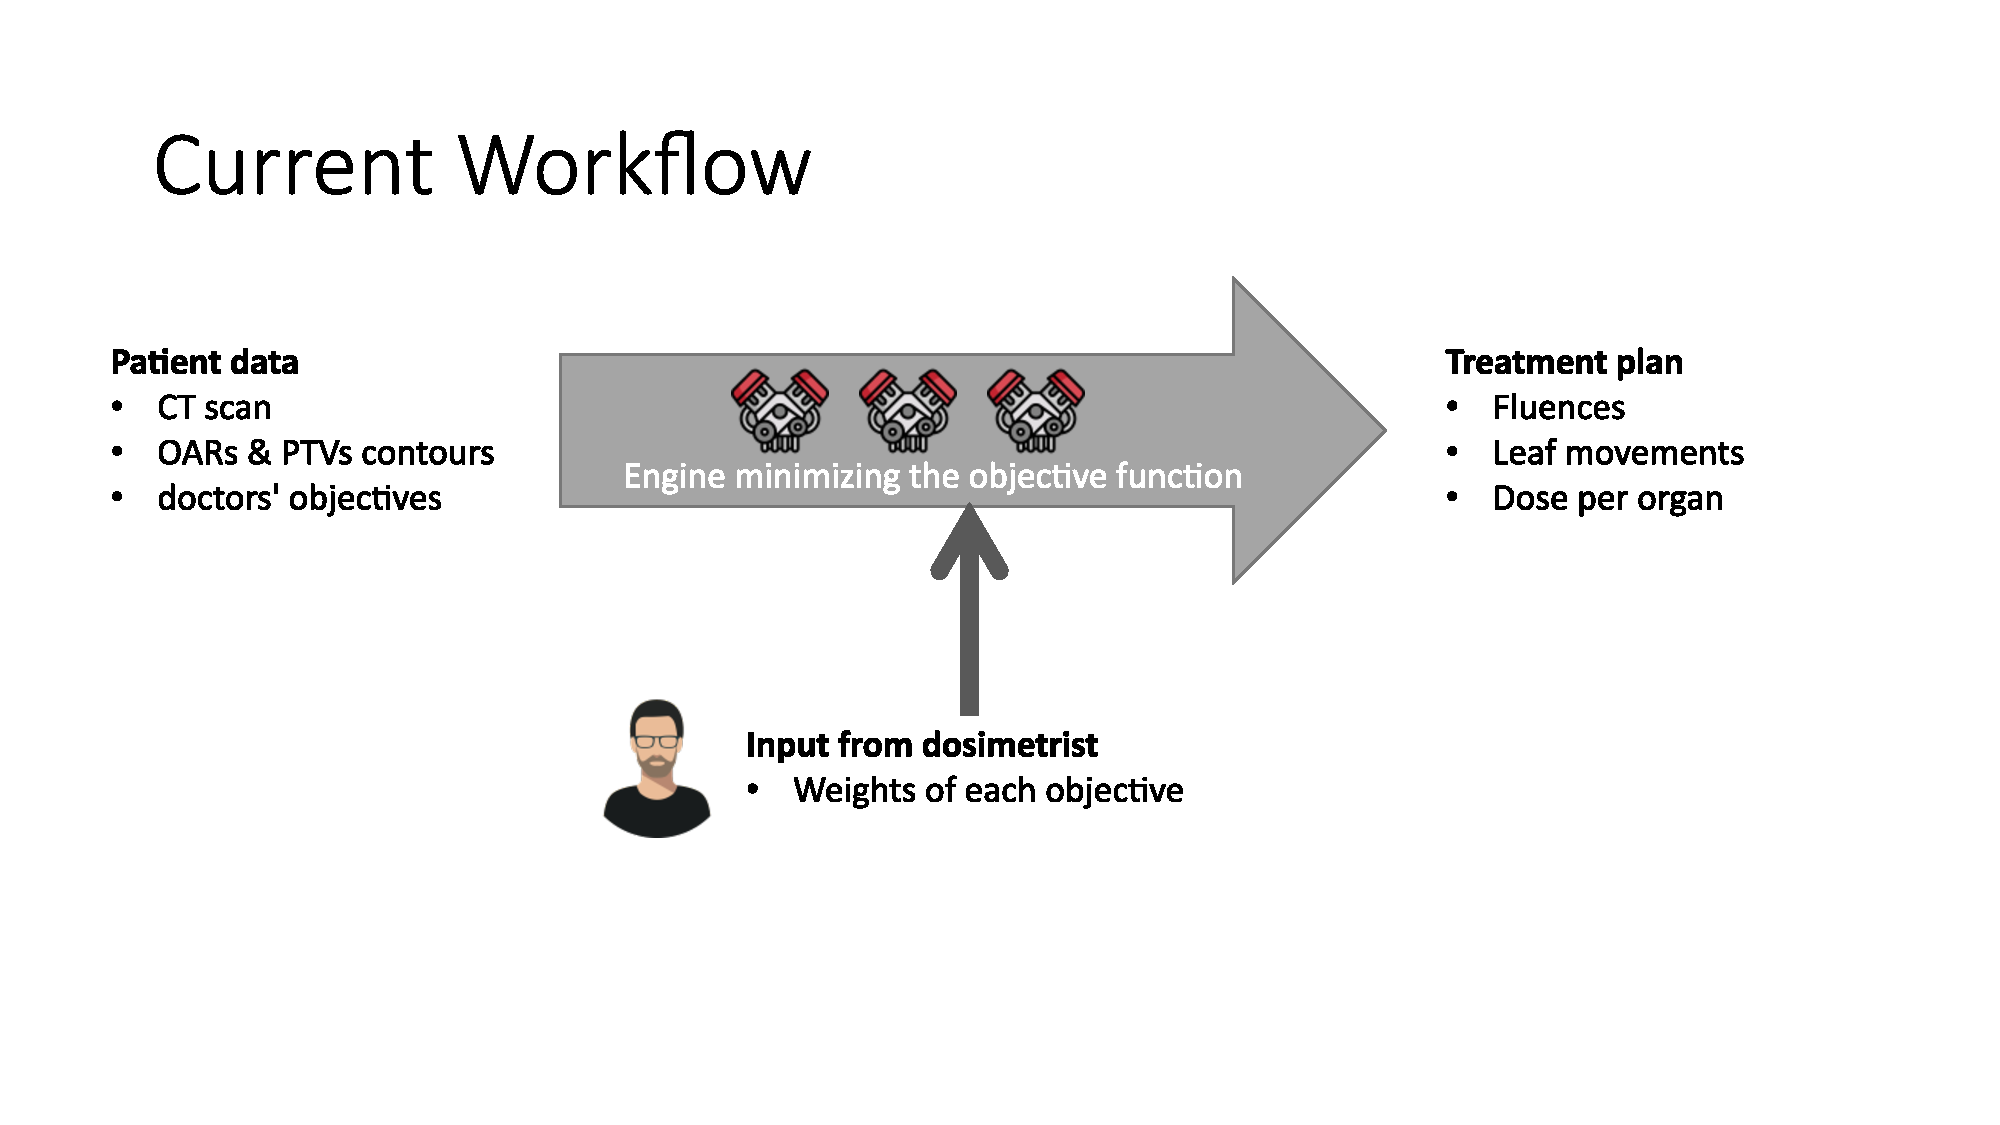
\includegraphics[width=\paperwidth]{imported_slides/current_workflow.pdf}}
	\end{frame}
	\begin{frame}
		\makebox[\linewidth]{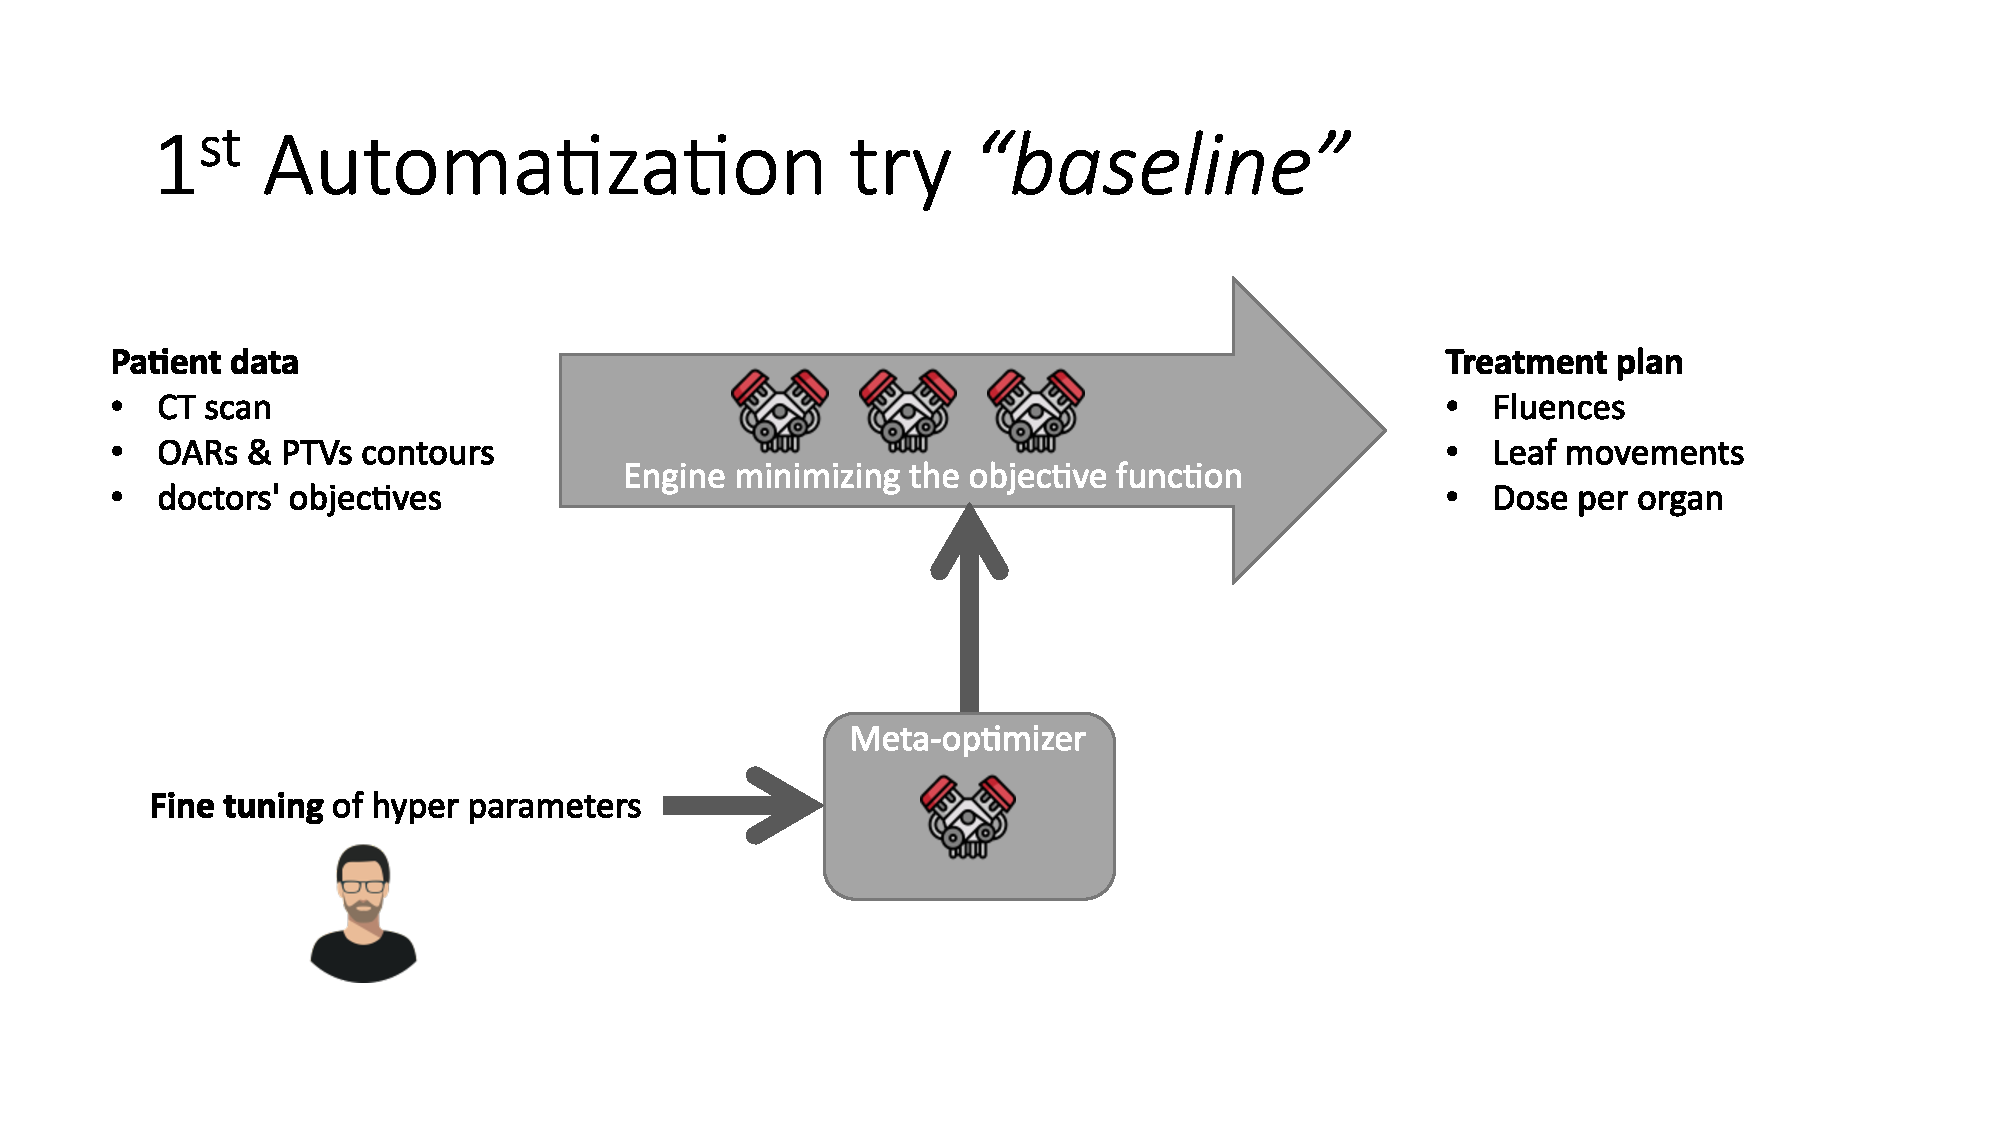
\includegraphics[width=\paperwidth]{imported_slides/metaoptim_workflow.pdf}}
	\end{frame}
	\begin{frame}
		\makebox[\linewidth]{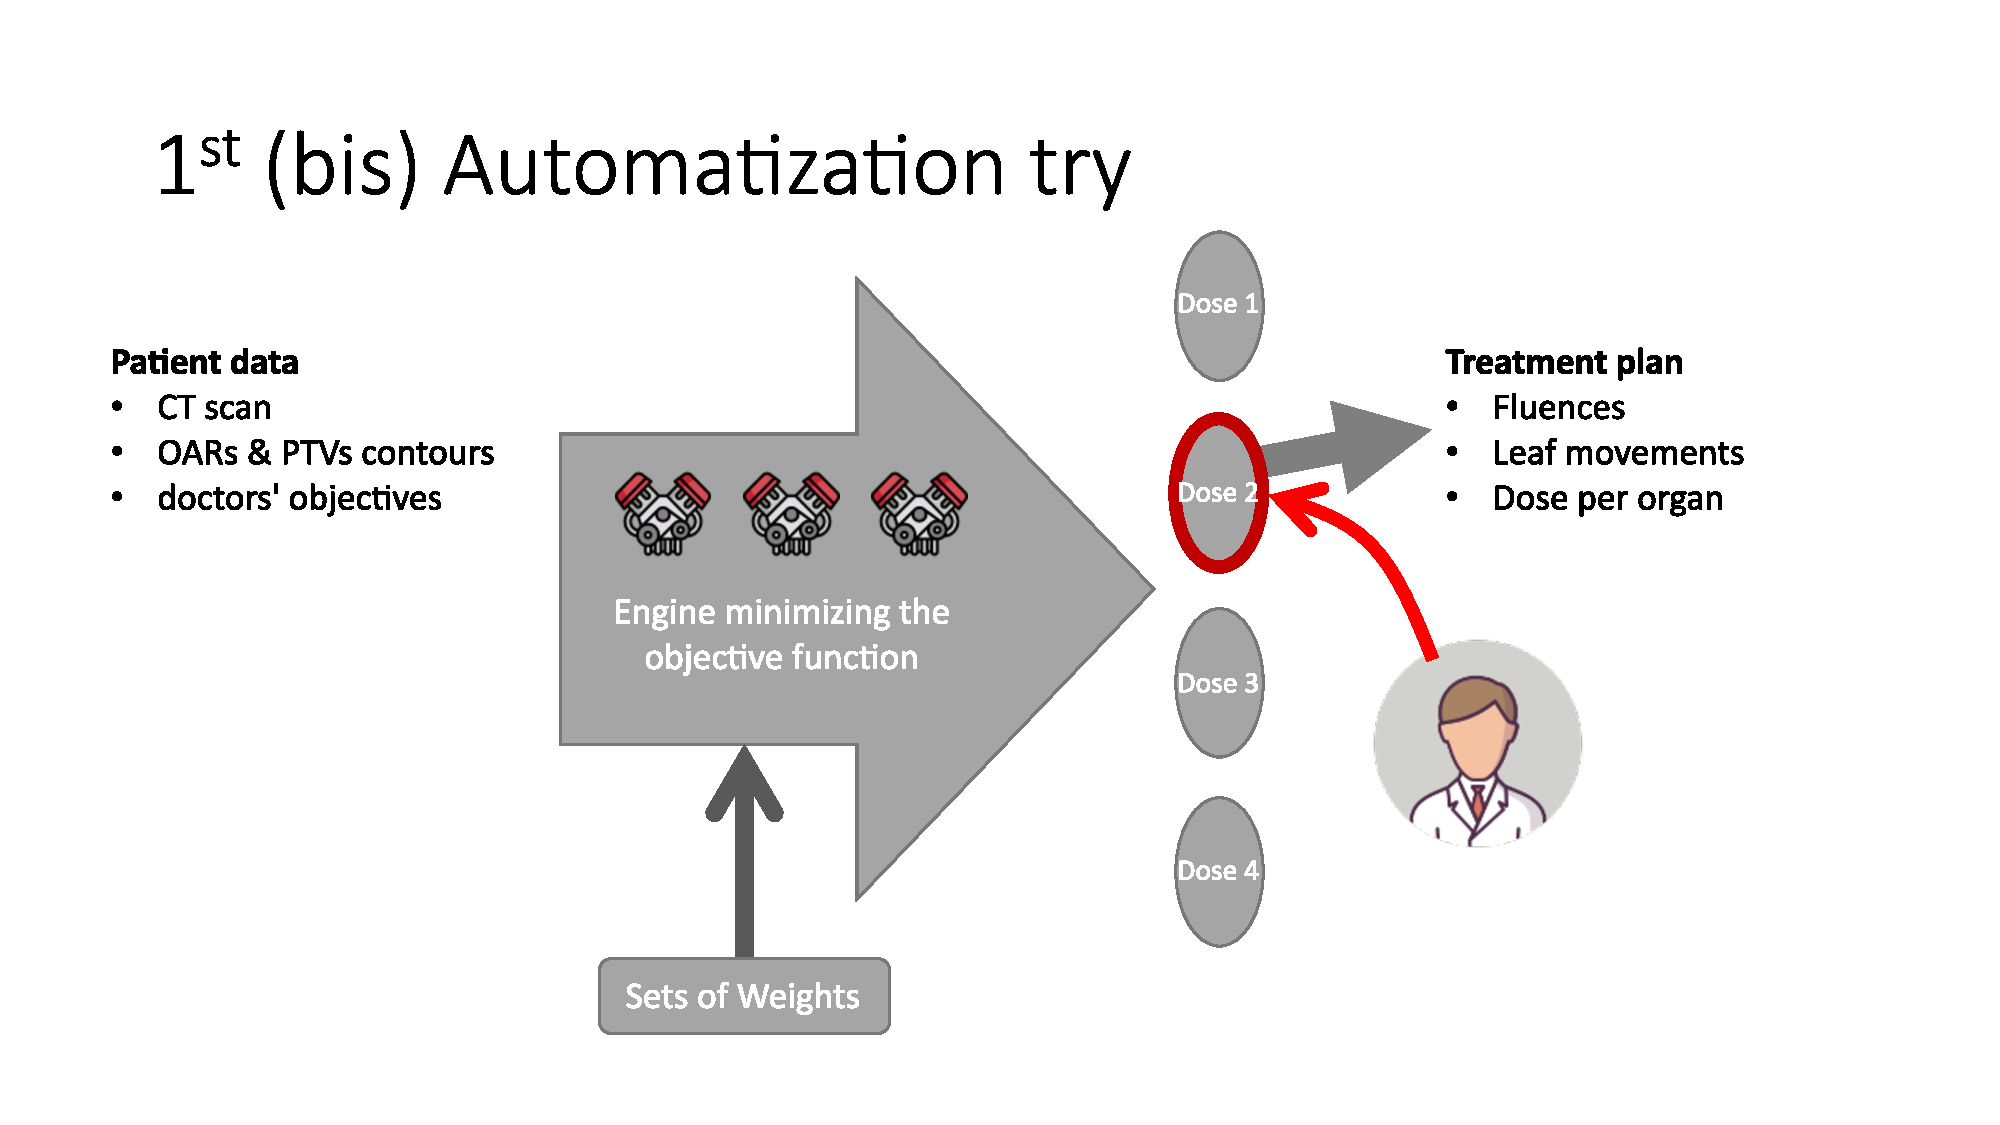
\includegraphics[width=\paperwidth]{imported_slides/clustering_workflow.pdf}}
	\end{frame}
	\begin{frame}
		\makebox[\linewidth]{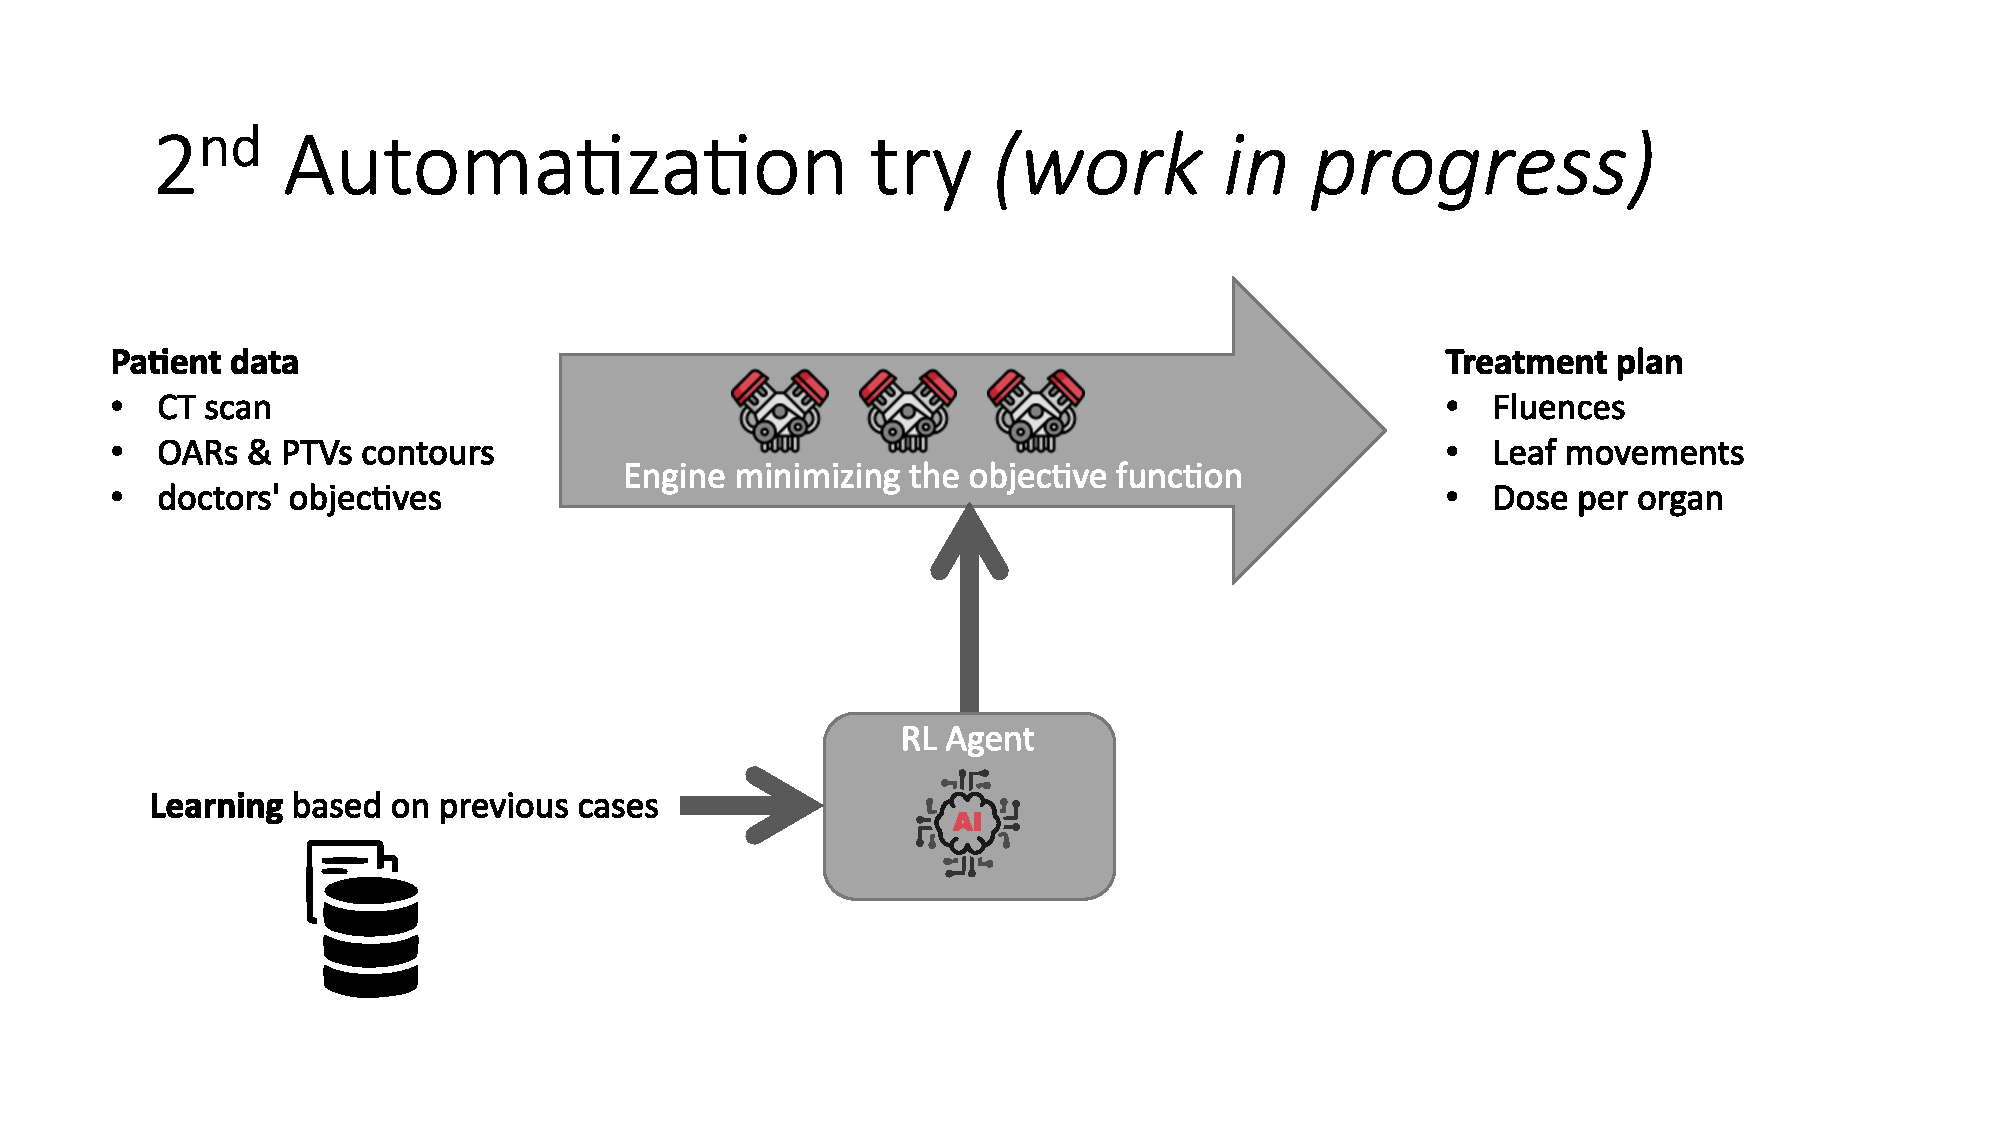
\includegraphics[width=\paperwidth]{imported_slides/rl_workflow.pdf}}
	\end{frame}
	% pareto appendix/workflow?
	
	\section{Future work}
	\subsection{Reinforcement Learning}
	\subsubsection{General Setup}
	\begin{frame}
		\frametitle{Reinforcement Learning Setup}
		\begin{itemize}
			\item [Agent] A network.
%			Agent: The agent is the learner or decision-maker that interacts with the environment. It takes actions based on the information it receives from the environment and learns to improve its decision-making abilities over time.
			\item [Env.] The current dose/weights, the CT scan, structures contours.
%			Environment: The environment is the external system or world in which the agent operates. It can be any environment where the agent needs to make sequential decisions, such as a game, a robot, or a simulated environment.
			\item [State] The agent will only access the the current dose/weights.
%			State: At each point in time, the environment is in a certain state, which represents a summary of the relevant information about the environment. The state can be fully observable or partially observable, depending on the available information to the agent.
			\item [Action] Changing the set of weights.
%			Action: The agent selects an action based on the current state it perceives from the environment. An action can be any decision or behavior the agent can take in a given state. The actions available to the agent depend on the specific problem and can be discrete or continuous.
			\item [Reward] The (DVH) distance between the current dose and the one that was actually used.
%			Reward: After taking an action, the agent receives feedback from the environment in the form of a reward signal. The reward represents the immediate desirability or quality of the action taken by the agent. The goal of the agent is to maximize the cumulative reward it receives over time.
			\item [Policy] The value changes of the sets of weights.
%			Policy: A policy is a mapping from states to actions, representing the agent's strategy or behavior. It determines the action the agent selects in a given state. Policies can be deterministic, meaning they directly map states to actions, or stochastic, meaning they provide a probability distribution over actions for each state.
		\end{itemize}
	\end{frame}
	\subsubsection{Planned Network Architecture}
	\begin{frame}
		\frametitle{Planned Network Architecture}
		\begin{figure}
			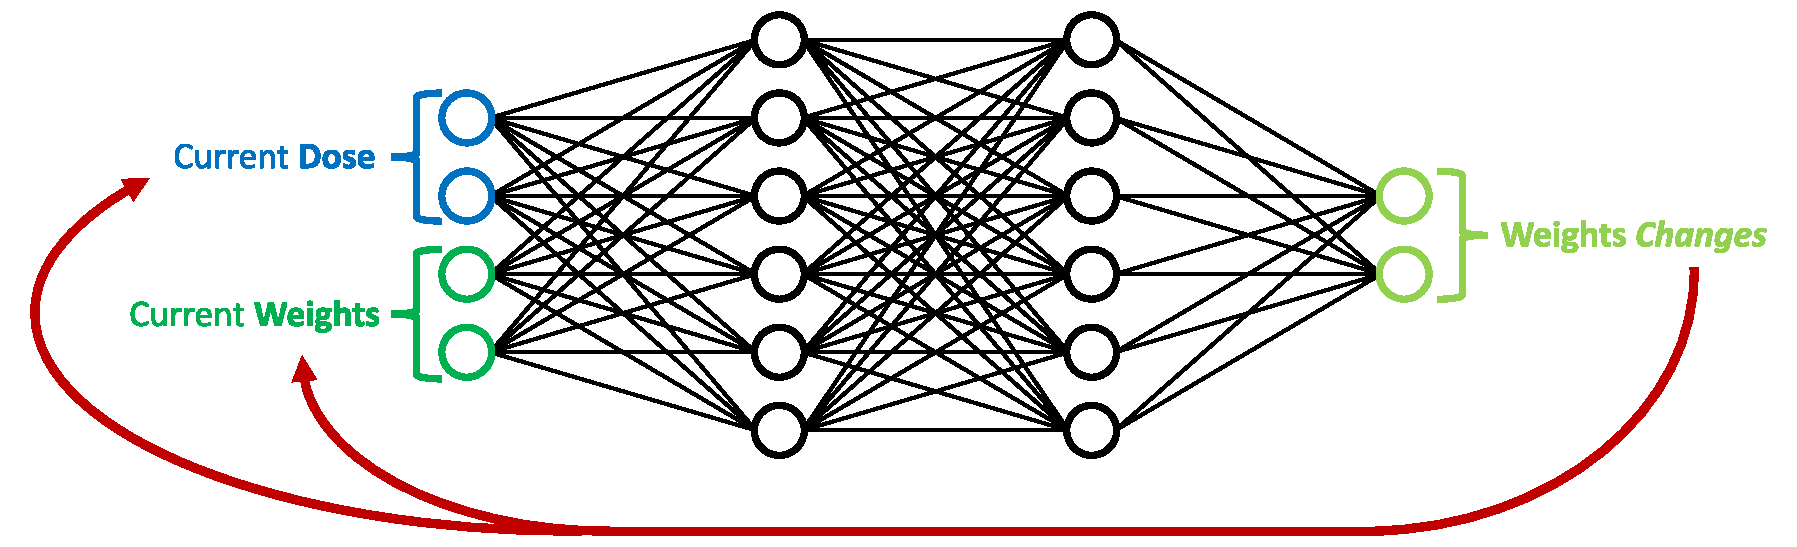
\includegraphics[width=\linewidth]{vector_images/rl_setup.pdf}
		\end{figure}
	\end{frame}
	\subsubsection{Trick}
	\begin{frame}
		\frametitle{Trick: encode the dose to smaller space}
		\begin{figure}
			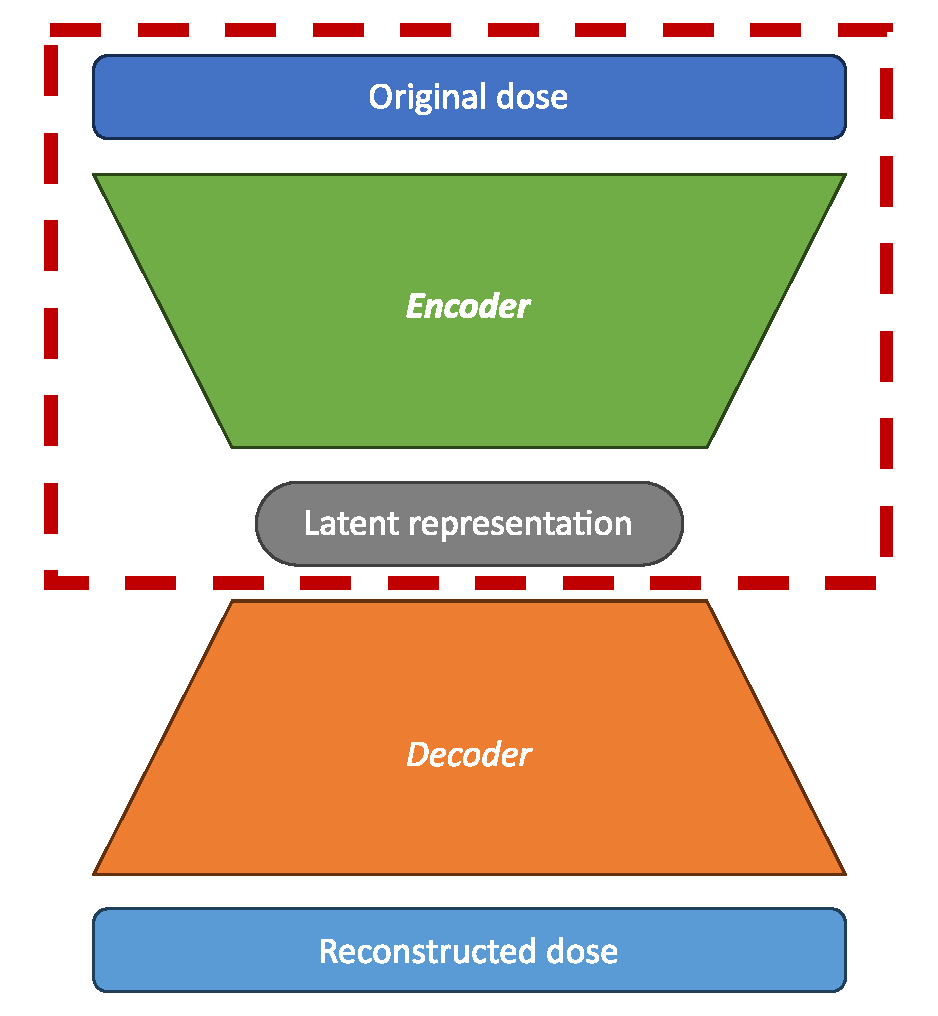
\includegraphics[height=6cm]{vector_images/dose_ae.pdf}
			\caption{Dose Auto-Encoder Architecture}
		\end{figure}
	\end{frame}
	\subsubsection{Challenges}
	\begin{frame}
		\frametitle{Challenges}
		\begin{itemize}
			\item normalize the body scan size
			\item normalize the structures per anatomy
			\item normalize the constraints per anatomy
		\end{itemize}
	\end{frame}
	% RL setup => normalization of constr; reward func
	
	\section{Others}
	\subsection{Teaching}
	\begin{frame}
		\frametitle{Teaching}
		Lectures:
		\begin{itemize}
			\item Mathematics Refresher Course for DSBA (M2 students) 2021
			\item Deep Learning for HSB (3\textsuperscript{rd} year students) 2023
		\end{itemize}
		\vspace{0.5cm}
		TDs:
		\begin{itemize}
			\item Coding Weeks (1\textsuperscript{st} year) 2021
			\item Optimization (1\textsuperscript{st} year) 2021
			\item Visual recognition (3\textsuperscript{rd} year) 2022
			\item Coding Weeks (1\textsuperscript{st} year) 2022
			\item Algorithm and Complexity (2\textsuperscript{nd} year) 2022/2023
		\end{itemize}
	\end{frame}
	
	\subsection{Doctoral Training}
	\begin{frame}
		\frametitle{Doctoral Training}
		\begin{itemize}
			\item ED INTERFACES - Journée de Rentrée 2022 (12 janvier 2023)
			\item Math On Mars (06 mai 2022) Info@lèze
			\item Asymmetric Cryptography (23 septembre 2022) Info@lèze
			\item Genetic Algorithms (10 juin 2022) Info@lèze
			\item Math With Jupyter (18 décembre 2021) Info@lèze
			\item Writing skills in Science ADVANCED [Eng] (10 mai 2022)
			\item AI 4 Health (10 janvier 2022 - 14 janvier 2022)
		\end{itemize}
		\vspace{0.5cm}
		Total participation: \textbf{109/125} heures; 7 modules\\
		Total des Crédits/Points de Thèse: \textbf{22/25}
	\end{frame}
	
	\section{References}
	\begin{frame}[allowframebreaks]
		\frametitle{References}
		\nocite{*}
		\bibliographystyle{plain}
		\bibliography{refs}
	\end{frame}

\end{document}